% This example is meant to be compiled with lualatex or xelatex
% The theme itself also supports pdflatex
\PassOptionsToPackage{unicode}{hyperref}
\documentclass[aspectratio=1610, xcolor=dvipsnames, 9pt]{beamer}

% Load packages you need here
\usepackage{polyglossia}
\setmainlanguage{german}

\usepackage{csquotes}
\usepackage{smartdiagram}

\usepackage{amsmath}
\usepackage{amssymb}
\usepackage{mathtools}

\usepackage{hyperref}
\usepackage{bookmark}

% load the theme after all packages

\usetheme[
  showtotalframes, % show total number of frames in the footline
]{fhswf}

% Put settings here, like
\unimathsetup{
  math-style=ISO,
  bold-style=ISO,
  nabla=upright,
  partial=upright,
  mathrm=sym,
}

\title{Neuronale Netze/Deep Learning und Predictive Maintenance}
\author[F.~Neubürger,]{ \textbf{Felix Neubürger}}
\institute[I \& W]{Fachhochschule Südwestfalen, Ingenieurs- \& Wirtschaftswissenschaften}
\date{01. Oktober 2025}
\titlegraphic{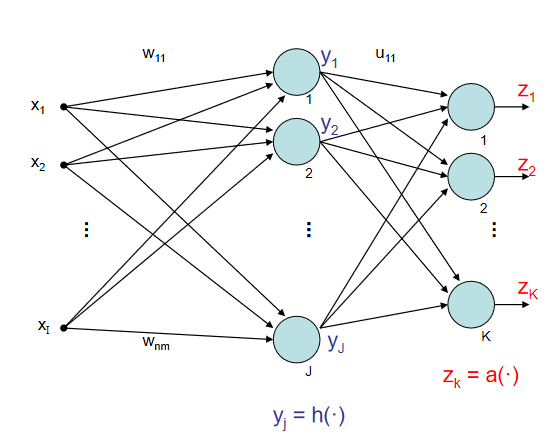
\includegraphics[width=0.2\textwidth]{images/MLP2.png}}


\begin{document}

\maketitle

\begin{frame}{Inhalte der Vorlesung}
  \begin{columns}
    \begin{column}{1\textwidth}
      \begin{itemize}
        \item \textbf{Mathematischer Refresher}: Lineare Algebra, Differentiation, Notation \newline
        \item \textbf{Grundlagen Neuronaler Netze}: Perceptron, Universal Approximation Theorem \newline
        \item \textbf{Mathematische Theorie}: Warum funktionieren neuronale Netze? \newline
        \item \textbf{Training und Optimierung}: Gradientenabstieg, Backpropagation, ADAM \newline
        \item \textbf{Deep Learning}: Vanishing Gradients, Aktivierungsfunktionen, tiefe Netze \newline
        \item \textbf{Spezielle Architekturen}: CNNs, RNNs, LSTMs, GANs, Autoencoders \newline

      \end{itemize}
    \end{column}
    \begin{column}{0\textwidth}
% \begin{figure}
% \centering
%             \includegraphics[width=0.9\textwidth]{images/intro/intro.pdf}
% \end{figure}
    \end{column}
  \end{columns}
\end{frame}

\begin{frame}{Ziele der Vorlesung - Welche Fragen sollen beantwortet werden?}
  \begin{columns}
    \begin{column}{0.69\textwidth}
      \begin{itemize}
        \item \textbf{Mathematisch}: Wie funktionieren neuronale Netze wirklich? \newline
        \item \textbf{Theoretisch}: Warum können sie jede Funktion approximieren? \newline
        \item \textbf{Praktisch}: Wie trainiert man sie effizient? \newline
        \item \textbf{Architektur}: Welche speziellen Netze für welche Probleme? \newline
        \item \textbf{Anwendung}: Wann ist Deep Learning die richtige Wahl? \newline
      \end{itemize}
    \end{column}
    \begin{column}{0.3\textwidth}
 \begin{figure}
 \centering
             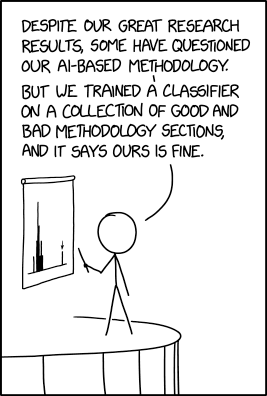
\includegraphics[width=0.9\textwidth]{images/ai_methodology.png}
             [\url{https://xkcd.com/2451/}]
 \end{figure}
    \end{column}
  \end{columns}
\end{frame}

\begin{frame}{Mathematischer Refresher -- Vektoren und Matrizen}
  \begin{columns}
    \begin{column}{1\textwidth}
      \begin{itemize}
        \item \textbf{Vektor}: Spaltenvektor $\mathbf{x} \in \mathbb{R}^d$ mit $d$ Komponenten
        \begin{equation}
          \mathbf{x} = \begin{pmatrix} x_1 \\\\ x_2 \\\\ \vdots \\\\ x_d \end{pmatrix}
        \end{equation}
        \item \textbf{Zeilenvektor}: $\mathbf{x}^T = (x_1, x_2, \ldots, x_d)$ (Transponiert)
        \item \textbf{Matrix}: $\mathbf{A} \in \mathbb{R}^{m \times n}$ mit $m$ Zeilen und $n$ Spalten
        \begin{equation}
          \mathbf{A} = \begin{pmatrix}
            a_{11} & a_{12} & \cdots & a_{1n} \\\\
            a_{21} & a_{22} & \cdots & a_{2n} \\\\
            \vdots & \vdots & \ddots & \vdots \\\\
            a_{m1} & a_{m2} & \cdots & a_{mn}
          \end{pmatrix}
        \end{equation}
        \item \textbf{Indexierung}: $a_{ij}$ = Element in Zeile $i$, Spalte $j$
      \end{itemize}
    \end{column}
  \end{columns}
\end{frame}

\begin{frame}{Mathematischer Refresher -- Grundoperationen}
  \begin{columns}
    \begin{column}{1\textwidth}
      \begin{itemize}
        \item \textbf{Skalarprodukt} (Dot Product): Für $\mathbf{x}, \mathbf{y} \in \mathbb{R}^d$
        \begin{equation}
          \mathbf{x}^T \mathbf{y} = \mathbf{x} \cdot \mathbf{y} = \sum_{i=1}^{d} x_i y_i
        \end{equation}
        \item \textbf{Matrix-Vektor-Multiplikation}: $\mathbf{A} \in \mathbb{R}^{m \times n}, \mathbf{x} \in \mathbb{R}^n$
        \begin{equation}
          \mathbf{y} = \mathbf{A}\mathbf{x} \in \mathbb{R}^m, \quad y_i = \sum_{j=1}^{n} a_{ij} x_j
        \end{equation}
        \item \textbf{Matrix-Matrix-Multiplikation}: $\mathbf{A} \in \mathbb{R}^{m \times k}, \mathbf{B} \in \mathbb{R}^{k \times n}$
        \begin{equation}
          \mathbf{C} = \mathbf{A}\mathbf{B} \in \mathbb{R}^{m \times n}, \quad c_{ij} = \sum_{\ell=1}^{k} a_{i\ell} b_{\ell j}
        \end{equation}
        \item \textbf{Elementweise Operationen}: Hadamard-Produkt $\mathbf{A} \odot \mathbf{B}$
        \begin{equation}
          (\mathbf{A} \odot \mathbf{B})_{ij} = a_{ij} \cdot b_{ij}
        \end{equation}
      \end{itemize}
    \end{column}
  \end{columns}
\end{frame}

\begin{frame}{Mathematischer Refresher -- Normen und Abstände}
  \begin{columns}
    \begin{column}{1\textwidth}
      \begin{itemize}
        \item \textbf{Euklidische Norm}: $||\mathbf{x}||_2 = \sqrt{\sum_{i=1}^{d} x_i^2}$ (Länge des Vektors)
        \item \textbf{L1-Norm}: $||\mathbf{x}||_1 = \sum_{i=1}^{d} |x_i|$ (Manhattan-Distanz)
        \item \textbf{Unendlich-Norm}: $||\mathbf{x}||_\infty = \max_i |x_i|$ (Maximum-Norm)
        \item \textbf{Frobenius-Norm} (für Matrizen): $||\mathbf{A}||_F = \sqrt{\sum_{i,j} a_{ij}^2}$
        \item \textbf{Einheitsvektor}: $\mathbf{u}$ mit $||\mathbf{u}||_2 = 1$
        \item \textbf{Orthogonale Vektoren}: $\mathbf{x} \perp \mathbf{y}$ wenn $\mathbf{x}^T \mathbf{y} = 0$
        \item \textbf{Linearkombination}: $\mathbf{y} = \alpha_1 \mathbf{x}_1 + \alpha_2 \mathbf{x}_2 + \ldots + \alpha_k \mathbf{x}_k$
      \end{itemize}
    \end{column}
  \end{columns}
\end{frame}

\begin{frame}{Mathematischer Refresher -- Differentiation und Gradienten}
  \begin{columns}
    \begin{column}{1\textwidth}
      \begin{itemize}
        \item \textbf{Partielle Ableitung}: Für $f: \mathbb{R}^n \to \mathbb{R}$
        \begin{equation}
          \frac{\partial f}{\partial x_i} = \lim_{h \to 0} \frac{f(\mathbf{x} + h\mathbf{e}_i) - f(\mathbf{x})}{h}
        \end{equation}
        \item \textbf{Gradient}: Vektor aller partiellen Ableitungen
        \begin{equation}
          \nabla f(\mathbf{x}) = \begin{pmatrix}
            \frac{\partial f}{\partial x_1} \\\\
            \frac{\partial f}{\partial x_2} \\\\
            \vdots \\\\
            \frac{\partial f}{\partial x_n}
          \end{pmatrix}
        \end{equation}
        \item \textbf{Kettenregel}: Für $f(g(x))$
        \begin{equation}
          \frac{d}{dx} f(g(x)) = f'(g(x)) \cdot g'(x)
        \end{equation}
        \item \textbf{Multivariable Kettenregel}: Für $f(\mathbf{u}(\mathbf{x}))$
        \begin{equation}
          \frac{\partial f}{\partial x_i} = \sum_j \frac{\partial f}{\partial u_j} \frac{\partial u_j}{\partial x_i} = \nabla_\mathbf{u} f \cdot \frac{\partial \mathbf{u}}{\partial x_i}
        \end{equation}
      \end{itemize}
    \end{column}
  \end{columns}
\end{frame}

\begin{frame}{Mathematischer Refresher -- Wichtige Funktionen und Eigenschaften}
  \begin{columns}
    \begin{column}{1\textwidth}
      \begin{itemize}
        \item \textbf{Exponentialfunktion}: $e^x$, Ableitung: $\frac{d}{dx} e^x = e^x$
        \item \textbf{Logarithmus}: $\ln(x)$, Ableitung: $\frac{d}{dx} \ln(x) = \frac{1}{x}$
        \item \textbf{Sigmoid-Funktion}: $\sigma(x) = \frac{1}{1 + e^{-x}}$
        \begin{equation}
          \sigma'(x) = \sigma(x)(1 - \sigma(x))
        \end{equation}
        \item \textbf{Quadratische Funktion}: $f(x) = ax^2 + bx + c$, Ableitung: $f'(x) = 2ax + b$
        \item \textbf{Produktregel}: $(fg)' = f'g + fg'$
        \item \textbf{Summenregel}: $(f + g)' = f' + g'$
        \item \textbf{Konstante Faktoren}: $(cf)' = cf'$ für Konstante $c$
      \end{itemize}
    \end{column}
  \end{columns}
\end{frame}

\begin{frame}{Mathematische Notation -- Überblick für diese Vorlesung}
  \begin{columns}
    \begin{column}{1\textwidth}
      \begin{itemize}
        \item \textbf{Skalare}: Kleinbuchstaben $a, b, c, x, y, z$
        \item \textbf{Vektoren}: Fettgedruckte Kleinbuchstaben $\mathbf{x}, \mathbf{y}, \mathbf{w}, \mathbf{b}$
        \item \textbf{Matrizen}: Fettgedruckte Großbuchstaben $\mathbf{A}, \mathbf{W}, \mathbf{X}$
        \item \textbf{Funktionen}: $f, g, h, L$ (Verlustfunktion)
        \item \textbf{Aktivierungsfunktionen}: $\sigma, \text{ReLU}, \tanh$
        \item \textbf{Indizes}:
        \begin{itemize}
          \item $i, j, k$: Datenindizes, Neuron-Indizes
          \item $(\ell)$: Schicht-Index, z.B. $\mathbf{W}^{(\ell)}$
          \item $(t)$: Zeit-/Iterationsindex, z.B. $\mathbf{w}^{(t)}$
        \end{itemize}
        \item \textbf{Wahrscheinlichkeiten}: $P, p, \mathbb{E}[\cdot]$ (Erwartungswert)
        \item \textbf{Approximation}: $\approx$, Proportionalität: $\propto$
      \end{itemize}
    \end{column}
  \end{columns}
\end{frame}


  \begin{frame}{Was sind Neuronale Netze und was ist Deep Learning?}
        \begin{columns}
          \begin{column}{0.7\textwidth}
            \begin{itemize}
              \item Abstrakt: Verkettung nichtlinearer Abbildungen \newline
              \item Die Parameter dieser Abbildungen wird mit vorhandenen Daten "gelernt" \newline
              \item Verschiedene Optimierungsverfahren zur Festlegung der "besten" Parameter \newline
            \end{itemize}
          \end{column}
          \begin{column}{0.3\textwidth}
       \begin{figure}
       \centering
                   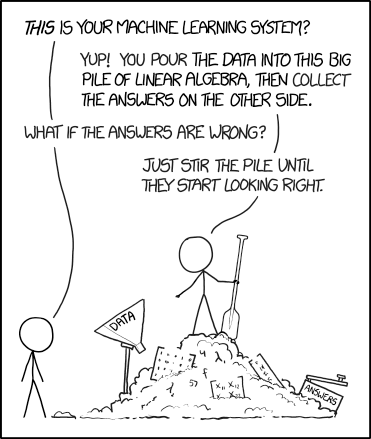
\includegraphics[width=0.9\textwidth]{images/machine_learning.png}\newline
             [\url{https://xkcd.com/1838/}]
       \end{figure}
          \end{column}
        \end{columns}
      \end{frame}

\begin{frame}{Warum funktionieren Neuronale Netze? -- Mathematische Intuition}
  \begin{columns}
    \begin{column}{1\textwidth}
      \begin{itemize}
        \item \textbf{Grundproblem}: Finde eine Funktion $f: \mathbb{R}^d \to \mathbb{R}^k$, die Eingaben $\mathbf{x}$ auf gewünschte Ausgaben $\mathbf{y}$ abbildet
        \item \textbf{Funktionsapproximation}: Neuronale Netze sind universelle Funktionsapproximatoren
        \item \textbf{Komposition einfacher Funktionen}: 
        \begin{equation}
          f(\mathbf{x}) = f_L \circ f_{L-1} \circ \ldots \circ f_2 \circ f_1(\mathbf{x})
        \end{equation}
        \item Jede Schicht $f_i$ führt eine \textbf{affine Transformation} gefolgt von \textbf{Nichtlinearität} aus:
        \begin{equation}
          f_i(\mathbf{x}) = \sigma_i(\mathbf{W}_i \mathbf{x} + \mathbf{b}_i)
        \end{equation}
        \item \textbf{Warum Nichtlinearität wichtig ist}: Ohne sie wäre das gesamte Netz nur eine lineare Transformation
        \begin{equation}
          \mathbf{W}_L(\mathbf{W}_{L-1}(\ldots(\mathbf{W}_1 \mathbf{x}))) = (\mathbf{W}_L \mathbf{W}_{L-1} \ldots \mathbf{W}_1) \mathbf{x} = \mathbf{W}_{\text{eff}} \mathbf{x}
        \end{equation}
      \end{itemize}
    \end{column}
  \end{columns}
\end{frame}

\begin{frame}{Warum funktionieren Neuronale Netze? -- Universal Approximation Theorem}
  \begin{columns}
    \begin{column}{1\textwidth}
      \begin{itemize}
        \item \textbf{Universal Approximation Theorem} \cite{cybenko1989,hornik1991}:
        \item Ein Feedforward-Netz mit einer versteckten Schicht kann jede stetige Funktion auf einem kompakten Definitionsbereich beliebig genau approximieren
        \item \textbf{Mathematische Formulierung}: Sei $\sigma: \mathbb{R} \to \mathbb{R}$ eine nicht-konstante, beschränkte und monotone Aktivierungsfunktion. Dann kann für jede stetige Funktion $g: [0,1]^d \to \mathbb{R}$ und $\epsilon > 0$ eine Funktion
        \begin{equation}
          F(\mathbf{x}) = \sum_{i=1}^N \alpha_i \sigma(\mathbf{w}_i^T \mathbf{x} + b_i)
        \end{equation}
        gefunden werden, sodass $|F(\mathbf{x}) - g(\mathbf{x})| < \epsilon$ für alle $\mathbf{x} \in [0,1]^d$
        \item \textbf{Praktische Bedeutung}: 
        \begin{itemize}
          \item Theoretisch können neuronale Netze jede Funktion lernen
          \item Problem: Anzahl der benötigten Neuronen kann exponentiell wachsen
          \item Deep Learning: Mehr Schichten können effizienter sein als breitere Netze
        \end{itemize}
      \end{itemize}
    \end{column}
  \end{columns}
\end{frame}

\begin{frame}{Die Mathematik des Lernens -- Warum Gradientenabstieg funktioniert}
  \begin{columns}
    \begin{column}{1\textwidth}
      \begin{itemize}
        \item \textbf{Optimierungsproblem}: Minimiere Verlustfunktion $L(\boldsymbol{\theta})$ über Parameter $\boldsymbol{\theta}$
        \item \textbf{Gradientenabstieg basiert auf Taylor-Entwicklung}:
        \begin{equation}
          L(\boldsymbol{\theta} + \boldsymbol{\Delta\theta}) \approx L(\boldsymbol{\theta}) + \nabla L(\boldsymbol{\theta})^T \boldsymbol{\Delta\theta}
        \end{equation}
        \item Um $L$ zu minimieren, wähle $\boldsymbol{\Delta\theta} = -\eta \nabla L(\boldsymbol{\theta})$ (mit $\eta > 0$)
        \item \textbf{Warum funktioniert das?} Für kleine $\eta$:
        \begin{equation}
          L(\boldsymbol{\theta} - \eta \nabla L(\boldsymbol{\theta})) \approx L(\boldsymbol{\theta}) - \eta ||\nabla L(\boldsymbol{\theta})||^2 \leq L(\boldsymbol{\theta})
        \end{equation}
        \item \textbf{Konvergenz-Eigenschaften}:
        \begin{itemize}
          \item Für konvexe Funktionen: Garantierte Konvergenz zum globalen Minimum
          \item Für nicht-konvexe Funktionen (neuronale Netze): Konvergenz zu lokalen Minima
          \item \textbf{Überraschung}: Lokale Minima sind oft "gut genug" für praktische Anwendungen
        \end{itemize}
      \end{itemize}
    \end{column}
  \end{columns}
\end{frame}
\begin{frame}{Konstruktion von Neuronalen Netzen: Single-Layer-Perceptron}
        \begin{columns}
          \begin{column}{0.7\textwidth}
            \begin{itemize}
              \item Einfacher binärer Klassifikator mit Aktivierungsfunktion
              \begin{equation}
                        f(\mathbf{x}) = \begin{cases}1 & \text{if }\ \mathbf{w}^T \mathbf{x} + b \geq \theta,\\0 & \text{otherwise}\end{cases}
                    \end{equation}
              \item mit dem Gewichtsvektor $\mathbf{w} \in \mathbb{R}^d$, Eingabevektor $\mathbf{x} \in \mathbb{R}^d$, Bias $b \in \mathbb{R}$ und Schwellwert $\theta$ \newline
              \item Das Skalarprodukt: $\mathbf{w}^T\mathbf{x} = \sum_{i=1}^{d} w_i x_i$ \newline
              \item Entscheidungsgrenze im 2D-Fall ($d=2$): Gerade mit Gleichung
              \begin{align}
                w_1 x_1 + w_2 x_2 + b &= \theta \\
                x_2 &= -\frac{w_1}{w_2} x_1 - \frac{b-\theta}{w_2}
              \end{align}
              \item Geometrische Interpretation: Hyperebene teilt den $\mathbb{R}^d$ in zwei Halbräume
              \item Linear separierbare Probleme: Klassen können durch Hyperebene getrennt werden
            \end{itemize}
          \end{column}
          \begin{column}{0.3\textwidth}
       \begin{figure}
       \centering
                   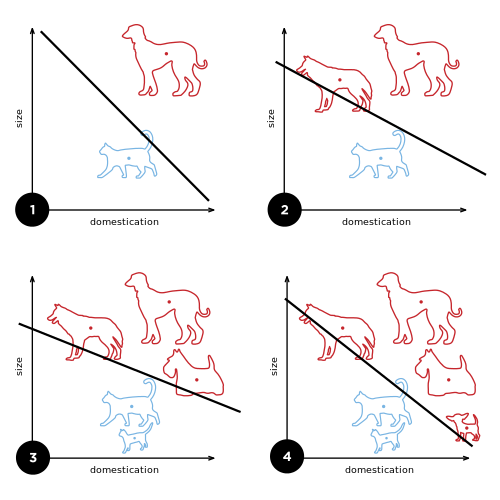
\includegraphics[width=0.9\textwidth]{images/Perceptron_example.svg.png}
       \end{figure}
          \end{column}
        \end{columns}
      \end{frame}

      \begin{frame}{Training von Neuronalen Netzen: Single-Layer-Perceptron}
        \begin{columns}
          \begin{column}{0.7\textwidth}
            \begin{itemize}
              \item Gegeben: Trainingsdatensatz $\mathcal{D} = \{(\mathbf{x}_i, y_i)\}_{i=1}^n$ mit $\mathbf{x}_i \in \mathbb{R}^d, y_i \in \{-1, +1\}$
              \item Perceptron-Lernregel \cite{rosenblatt1958}:
                    \begin{equation}
                       \mathbf{w}^{(t+1)} = \mathbf{w}^{(t)} + \eta \sum_{(\mathbf{x}_i, y_i) \in \mathcal{M}^{(t)}} y_i \mathbf{x}_i
                    \end{equation}
              \item Fehlklassifizierungen: $\mathcal{M}^{(t)} = \{(\mathbf{x}_i, y_i) : y_i(\mathbf{w}^{(t)T}\mathbf{x}_i + b) \leq 0\}$
              \item Verlustfunktion (Perceptron-Verlust):
              \begin{equation}
                L(\mathbf{w}, b) = \sum_{(\mathbf{x}_i, y_i) \in \mathcal{M}} -y_i(\mathbf{w}^T\mathbf{x}_i + b)
              \end{equation}
              \item Konvergenz-Theorem: Für linear separierbare Daten konvergiert der Algorithmus in endlich vielen Schritten
              \item Margin $\gamma = \min_{i} \frac{y_i(\mathbf{w}^*T\mathbf{x}_i + b^*)}{||\mathbf{w}^*||_2}$ bestimmt Konvergenzgeschwindigkeit
            \end{itemize}
          \end{column}
          \begin{column}{0.3\textwidth}
       \begin{figure}
       \centering
                   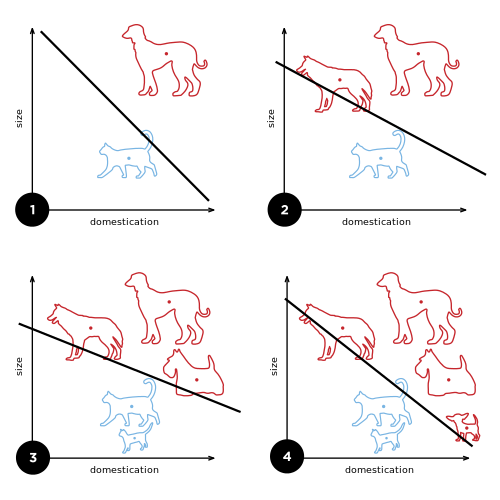
\includegraphics[width=0.9\textwidth]{images/Perceptron_example.svg.png}
       \end{figure}
          \end{column}
        \end{columns}
      \end{frame}

      \begin{frame}{Training von Neuronalen Netzen: Gradientenabstieg}
        \begin{columns}
          \begin{column}{0.7\textwidth}
            \begin{itemize}
              \item \textbf{Gradientenabstieg} (Gradient Descent) - allgemeines Optimierungsverfahren
              \item Iterative Aktualisierung der Parameter:
                    \begin{equation}
                       \boldsymbol{\theta}^{(t+1)} = \boldsymbol{\theta}^{(t)} - \eta \nabla_{\boldsymbol{\theta}} L(\boldsymbol{\theta}^{(t)})
                    \end{equation}
              \item $\eta > 0$: Lernrate (Schrittweite), $\boldsymbol{\theta}$: Parametervektor
              \item Gradient einer Funktion $f: \mathbb{R}^n \to \mathbb{R}$:
              \begin{equation}
                \nabla f(\mathbf{x}) = \left( \frac{\partial f}{\partial x_1}, \frac{\partial f}{\partial x_2}, \ldots, \frac{\partial f}{\partial x_n} \right)^T
              \end{equation}
              \item Gradient zeigt in Richtung des steilsten Anstiegs $\Rightarrow$ $-\nabla f$ zeigt zum lokalen Minimum
              \item Für Perceptron-Verlust: 
              \begin{align}
                \frac{\partial L}{\partial w_j} &= \sum_{(\mathbf{x}_i, y_i) \in \mathcal{M}} -y_i x_{ij} \\
                \nabla_{\mathbf{w}} L &= -\sum_{(\mathbf{x}_i, y_i) \in \mathcal{M}} y_i \mathbf{x}_i
              \end{align}
            \end{itemize}
          \end{column}
          \begin{column}{0.3\textwidth}
       \begin{figure}
       \centering
                   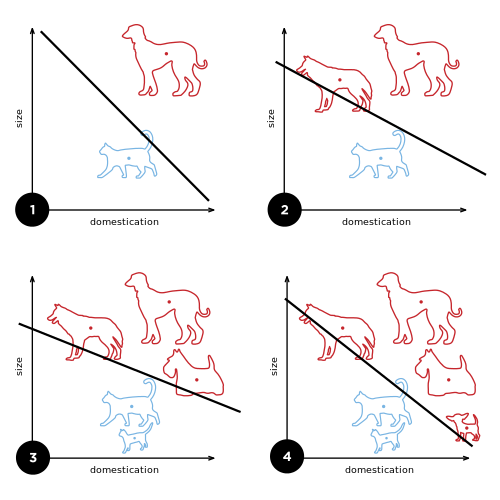
\includegraphics[width=0.9\textwidth]{images/Perceptron_example.svg.png}
       \end{figure}
          \end{column}
        \end{columns}
      \end{frame}

      \begin{frame}{Training von Neuronalen Netzen: Single-Layer-Perceptron}
        \begin{columns}
          \begin{column}{0.7\textwidth}
            \begin{itemize}

              \item Daraus folgt: \begin{align} 
                                  \nabla f(w) &= \left(  -\sum_{x \in F(w)} x_1,  -\sum_{x \in F(w)} x_2, ... ,  -\sum_{x \in F(w)} x_n   \right)
                                              &= -\sum_{x \in F(w)} x
                                  \end{align}
            \end{itemize}
          \end{column}
          \begin{column}{0.3\textwidth}
       \begin{figure}
       \centering
                   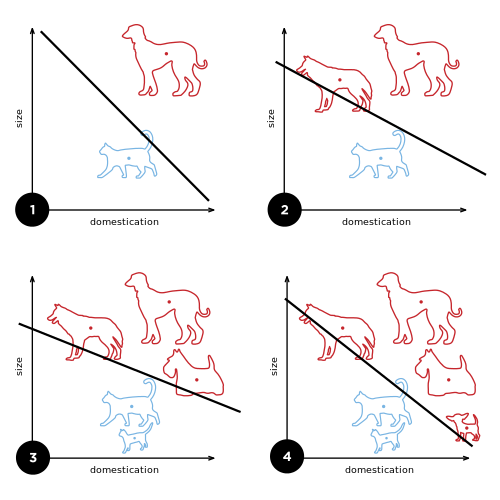
\includegraphics[width=0.9\textwidth]{images/Perceptron_example.svg.png}
       \end{figure}
          \end{column}
        \end{columns}
      \end{frame}

\begin{frame}{Grenzen des Single-Layer-Perceptrons -- Das XOR-Problem}
  \begin{columns}
    \begin{column}{0.6\textwidth}
      \begin{itemize}
        \item \textbf{Fundamentale Limitation}: Perceptron kann nur linear separierbare Probleme lösen
        \item \textbf{XOR-Problem} \cite{minsky1969}: 
        \begin{center}
        \begin{tabular}{|c|c|c|}
        \hline
        $x_1$ & $x_2$ & XOR \\
        \hline
        0 & 0 & 0 \\
        0 & 1 & 1 \\
        1 & 0 & 1 \\
        1 & 1 & 0 \\
        \hline
        \end{tabular}
        \end{center}
        \item \textbf{Mathematischer Beweis der Unmöglichkeit}: 
        \item Angenommen, es existiert $\mathbf{w} = (w_1, w_2)$ und $b$, sodass:
        \begin{align}
          w_1 \cdot 0 + w_2 \cdot 1 + b &> 0 \quad \text{(für (0,1))} \\
          w_1 \cdot 1 + w_2 \cdot 0 + b &> 0 \quad \text{(für (1,0))} \\
          w_1 \cdot 0 + w_2 \cdot 0 + b &\leq 0 \quad \text{(für (0,0))} \\
          w_1 \cdot 1 + w_2 \cdot 1 + b &\leq 0 \quad \text{(für (1,1))}
        \end{align}
        \item Aus (1) und (3): $w_2 > -b \geq 0 \Rightarrow w_2 > 0$
        \item Aus (2) und (3): $w_1 > -b \geq 0 \Rightarrow w_1 > 0$
        \item Aber (4): $w_1 + w_2 + b \leq 0$ \textbf{Widerspruch!}
      \end{itemize}
    \end{column}
    \begin{column}{0.4\textwidth}
      \begin{figure}
        \centering
                    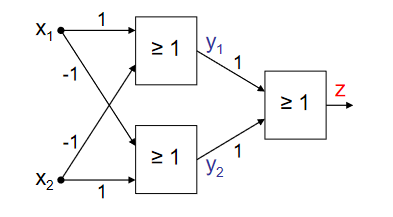
\includegraphics[width=0.9\textwidth]{images/XOR.png}
        \end{figure}
    \end{column}
  \end{columns}
\end{frame}

      \begin{frame}{Konstruktion von Neuronalen Netzen: Multi-Layer-Perceptron}
        \begin{columns}
          \begin{column}{0.7\textwidth}
            \begin{itemize}
              \item \textbf{Lösung des XOR-Problems}: Mehrschichtige Netze!
              \item \textbf{Komposition von Hyperebenen}: 
              \begin{itemize}
                \item Erste Schicht: Erzeugt mehrere lineare Entscheidungsgrenzen
                \item Zweite Schicht: Kombiniert diese zu komplexeren Formen
              \end{itemize}
              \item \textbf{Mathematische Intuition für XOR}:
              \begin{align}
                h_1 &= \sigma(x_1 + x_2 - 0.5) \quad \text{(OR-Gate)} \\
                h_2 &= \sigma(-x_1 - x_2 + 1.5) \quad \text{(NAND-Gate)} \\
                \text{XOR} &= \sigma(h_1 + h_2 - 1.5)
              \end{align}
              \item \textbf{Universal Approximation}: Mit einer versteckten Schicht können beliebige stetige Funktionen approximiert werden
              \item \textbf{Tiefe vs. Breite}: Tiefere Netze können effizienter sein als breitere
            \end{itemize}
          \end{column}
          \begin{column}{0.3\textwidth}
            \begin{figure}
              \centering
                          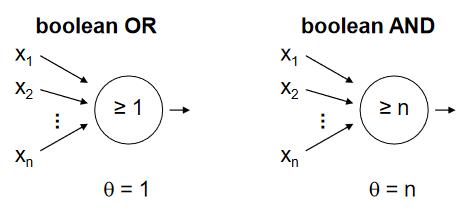
\includegraphics[width=0.9\textwidth]{images/OR_AND.png}
              \end{figure}
       \begin{figure}
       \centering
                   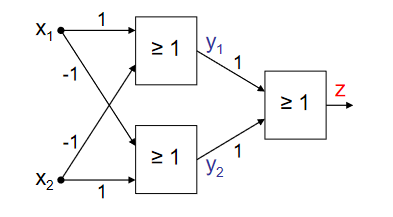
\includegraphics[width=0.9\textwidth]{images/XOR.png}
       \end{figure}
          \end{column}
        \end{columns}
      \end{frame}

      \begin{frame}{Training von Neuronalen Netzen: Multi-Layer-Perceptron}
        \begin{columns}
          \begin{column}{0.7\textwidth}
            \begin{itemize}
              \item \textbf{Multilayer Perceptron (MLP)}: Neuronales Netz mit versteckten Schichten
              \item Forward-Pass für 2-Schicht-Netz:
              \begin{align}
                \mathbf{z}^{(1)} &= \mathbf{W}^{(1)} \mathbf{x} + \mathbf{b}^{(1)} \quad \text{(lineare Transformation)} \\
                \mathbf{a}^{(1)} &= \sigma(\mathbf{z}^{(1)}) \quad \text{(Aktivierung)} \\
                \mathbf{z}^{(2)} &= \mathbf{W}^{(2)} \mathbf{a}^{(1)} + \mathbf{b}^{(2)} \\
                \hat{\mathbf{y}} &= \sigma(\mathbf{z}^{(2)})
              \end{align}
              \item Mean Squared Error (MSE) Loss:
              \begin{equation}
                L(\mathbf{W}, \mathbf{b}) = \frac{1}{n} \sum_{i=1}^{n} ||\hat{\mathbf{y}}_i - \mathbf{y}_i||_2^2
              \end{equation}
              \item Problem der Heaviside-Funktion: $H(x) = \begin{cases}1 & x \geq 0\\0 & x < 0\end{cases}$ nicht differenzierbar
              \item Lösung: Glatte Aktivierungsfunktionen (Sigmoid, Tanh, ReLU)
            \end{itemize}
          \end{column}
          \begin{column}{0.3\textwidth}
            \begin{figure}
              \centering
                          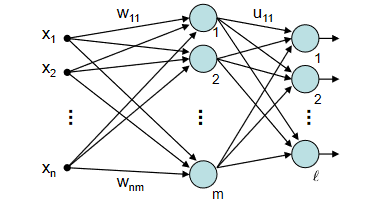
\includegraphics[width=0.9\textwidth]{images/MLP.png}
              \end{figure}
          \end{column}
        \end{columns}
      \end{frame}

      \begin{frame}{Training von Neuronalen Netzen: Multi-Layer-Perceptron}
        \begin{columns}
          \begin{column}{0.7\textwidth}
            \begin{itemize}
              \item
              \begin{equation}
                f(w) = \sum_{x\in B} || g(w; x) - g^*(x) ||^2 \quad \rightarrow \text{  min  }
              \end{equation} 
              \item mit dem Output des Netzes $ g(w;x) $ und dem erwarteten Output $ g^*(x) $ 
              \item 
              \begin{align}
                 u^{(t+1)} &= u^t - \gamma \nabla_u f(w_t , u_t) \\
                 w^{(t+1)} &= w^t - \gamma \nabla_w f(w_t , u_t) \\
              \end{align}
              \item $x_i$: Inputs 
              \item $y_j$: Werte nach dem ersten Layer
              \item $z_k$: Werte nach dem zweiten Layer
            \end{itemize}
          \end{column}
          \begin{column}{0.3\textwidth}
            \begin{figure}
              \centering
                          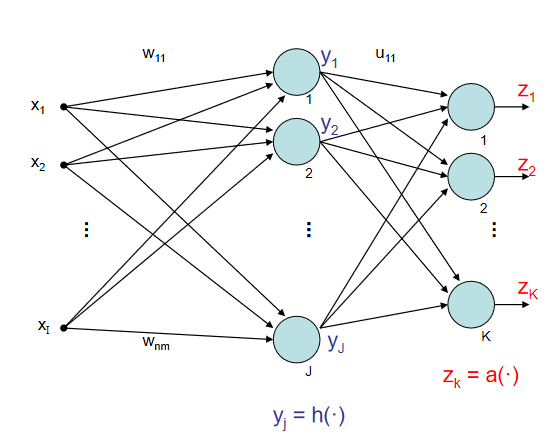
\includegraphics[width=0.9\textwidth]{images/MLP2.png}
              \end{figure}
          \end{column}
        \end{columns}
      \end{frame}

      \begin{frame}{Backpropagation: Grundidee}
        \begin{columns}
          \begin{column}{1\textwidth}
            \begin{itemize}
              \item \textbf{Backpropagation} \cite{rumelhart1986}: Effizienter Algorithmus zur Berechnung von Gradienten
              \item \textbf{Problem}: Wie berechnen wir $\frac{\partial L}{\partial w_{ij}}$ in tiefen Netzen?
              \item \textbf{Lösung}: Anwendung der \textbf{Kettenregel} der Differentiation:
              \begin{equation}
                \frac{\partial L}{\partial w_{ij}^{(l)}} = \frac{\partial L}{\partial z_j^{(l)}} \cdot \frac{\partial z_j^{(l)}}{\partial w_{ij}^{(l)}}
              \end{equation}
              \item Definition der \textbf{lokalen Gradienten} (Deltas):
              \begin{equation}
                \delta_j^{(l)} = \frac{\partial L}{\partial z_j^{(l)}}
              \end{equation}
              \item \textbf{Idee}: Berechne Fehler rückwärts durch das Netz
            \end{itemize}
          \end{column}
        \end{columns}
      \end{frame}

      \begin{frame}{Backpropagation: Algorithmus}
        \begin{columns}
          \begin{column}{1\textwidth}
            \begin{itemize}
              \item \textbf{Forward Pass}: Berechne Ausgaben für alle Schichten
              \item \textbf{Backward Pass}: Berechne Gradienten rekursiv
              \item \textbf{Output-Schicht}:
              \begin{equation}
                \delta_j^{(L)} = \frac{\partial L}{\partial a_j^{(L)}} \cdot \sigma'(z_j^{(L)})
              \end{equation}
              \item \textbf{Versteckte Schichten}:
              \begin{equation}
                \delta_j^{(l)} = \left(\sum_{k} \delta_k^{(l+1)} w_{jk}^{(l+1)}\right) \sigma'(z_j^{(l)})
              \end{equation}
              \item \textbf{Gradientenberechnung}:
              \begin{align}
                \frac{\partial L}{\partial w_{ij}^{(l)}} &= \delta_j^{(l)} \cdot a_i^{(l-1)} \\
                \frac{\partial L}{\partial b_j^{(l)}} &= \delta_j^{(l)}
              \end{align}
            \end{itemize}
          \end{column}
        \end{columns}
      \end{frame}

      \begin{frame}{MLP Training: Grundlagen}
        \begin{columns}
          \begin{column}{1\textwidth}
            \begin{itemize}
              \item Analog zum SLP: Gradientenabstieg zur Fehlerminimierung
              \item \textbf{Batch-Gradient}:
              \begin{align}
                \nabla f(w,u) &= \sum_{x,z^* \in B} \nabla f(w, u; x,z^*)
              \end{align}
              \item \textbf{Sigmoid-Aktivierungsfunktion}:
              \begin{align}
                \sigma(x) = \frac{1}{1+e^{-x}} \quad \text{mit} \quad \sigma'(x) = \sigma(x) \cdot (1 - \sigma(x))
              \end{align}
              \item \textbf{Kettenregel}:
              \begin{equation}
                [f(g(x))]' = f'(g(x)) \cdot g'(x)
              \end{equation}
              \item \textbf{Fehlerterm} (Delta): $\delta_j = \frac{\partial L}{\partial z_j}$
            \end{itemize}
          \end{column}
        \end{columns}
      \end{frame}

      \begin{frame}{MLP Training: Gradientenberechnung Output-Schicht}
        \begin{columns}
          \begin{column}{1\textwidth}
            \begin{itemize}
              \item \textbf{Fehlerterm für Output-Schicht}:
              \begin{align}
                \delta_k^{(out)} &= \frac{\partial L}{\partial z_k^{(out)}} \\
                &= 2(z_k - z_k^*) \cdot \sigma'(z_k^{(out)}) \\
                &= 2(z_k - z_k^*) \cdot z_k \cdot (1 - z_k)
              \end{align}
              \item \textbf{Gradient für Output-Gewichte}:
              \begin{align}
                \frac{\partial L}{\partial u_{jk}} &= \delta_k^{(out)} \cdot y_j
              \end{align}
              \item Wobei $y_j$ die Aktivierung der versteckten Schicht ist
            \end{itemize}
          \end{column}
        \end{columns}
      \end{frame}
      \begin{frame}{MLP Training: Gradientenberechnung versteckte Schicht}
        \begin{columns}
          \begin{column}{1\textwidth}
            \begin{itemize}
              \item \textbf{Fehlerterm für versteckte Schicht}:
              \begin{align}
                \delta_j^{(hidden)} &= \frac{\partial L}{\partial z_j^{(hidden)}} \\
                &= \sum_{k} \delta_k^{(out)} \cdot u_{jk} \cdot \sigma'(z_j^{(hidden)}) \\
                &= y_j (1-y_j) \sum_{k} \delta_k^{(out)} \cdot u_{jk}
              \end{align}
              \item \textbf{Gradient für versteckte Gewichte}:
              \begin{align}
                \frac{\partial L}{\partial w_{ij}} &= \delta_j^{(hidden)} \cdot x_i
              \end{align}
              \item \textbf{Backpropagation}: Fehler propagiert rückwärts!
            \end{itemize}
          \end{column}
        \end{columns}
      \end{frame}

      \begin{frame}{ Verallgemeinerung Training von Neuronalen Netzen: M-Layer-Perceptron}
        \begin{columns}
          \begin{column}{1\textwidth}
            \begin{itemize}
              \item bei einem Neuronalen Netz mi $L$ Layern $S_1, S_2 , ... , S_L$
              \item den Gewichten $w_{ij}$ in der Matrix $W$
              \item dem output eines Neurons $o_j$
              \item ist der Fehlerterm: 
            \begin{equation*}
              \delta_j = \begin{cases} o_j \cdot (1-o_j) \cdot  (o_j -z_j*) & \text{if }\ j \in S_L, \text{output Neuron} \\ o_j \cdot (1-o_j) \cdot \sum_{k \in S_{m+1}} \delta_k \cdot w_{jk} & \text{if } j \in S_m \text{and } m<L \end{cases}
            \end{equation*}
            \item Der Korrekturterm für die einzelnen Gewichte ist dann:
            \begin{equation}
              w_{ij}^{(t+1)} = w_{ij}^{t} - \gamma \cdot o_i \cdot \delta_j 
            \end{equation}
            \end{itemize}
          \end{column}
          %\begin{column}{0.3\textwidth}
          %  \begin{figure}
          %    \centering
          %                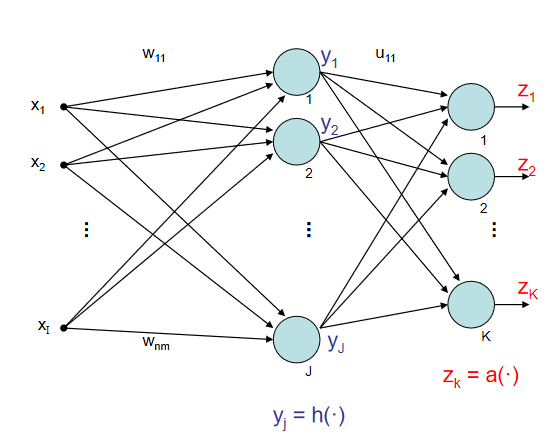
\includegraphics[width=0.9\textwidth]{images/MLP2.png}
          %    \end{figure}
          %\end{column}
        \end{columns}
      \end{frame}

      \begin{frame}{Fortgeschrittene Optimierungsalgorithmen}
        \begin{columns}
          \begin{column}{1\textwidth}
            \begin{itemize}
              \item \textbf{Momentum}: Beschleunigung in konsistente Richtungen
              \begin{align}
                \mathbf{v}^{(t+1)} &= \beta \mathbf{v}^{(t)} + \eta \nabla L(\boldsymbol{\theta}^{(t)}) \\
                \boldsymbol{\theta}^{(t+1)} &= \boldsymbol{\theta}^{(t)} - \mathbf{v}^{(t+1)}
              \end{align}
              \item \textbf{ADAM} \cite{kingma2014adam} (Adaptive Moment Estimation) - Kombination aus Momentum und RMSprop:
              \begin{align}
                m_w^{(t+1)} &= \beta_1 m_w^{(t)} + (1 - \beta_1) \nabla_w L^{(t)} \quad \text{(1. Moment)} \\
                v_w^{(t+1)} &= \beta_2 v_w^{(t)} + (1 - \beta_2) (\nabla_w L^{(t)})^2 \quad \text{(2. Moment)} \\
                \hat{m}_w^{(t)} &= \frac{m_w^{(t+1)}}{1 - \beta_1^{t+1}} \quad \text{(Bias-Korrektur)} \\
                \hat{v}_w^{(t)} &= \frac{v_w^{(t+1)}}{1 - \beta_2^{t+1}} \quad \text{(Bias-Korrektur)} \\
                w^{(t+1)} &= w^{(t)} - \frac{\eta}{\sqrt{\hat{v}_w^{(t)}} + \epsilon} \hat{m}_w^{(t)}
              \end{align}
              \item Typische Hyperparameter: $\beta_1 = 0.9$, $\beta_2 = 0.999$, $\epsilon = 10^{-8}$
            \end{itemize}
          \end{column}
          % \begin{column}{0.3\textwidth}
          %   \begin{figure}
          %     \centering
          %                 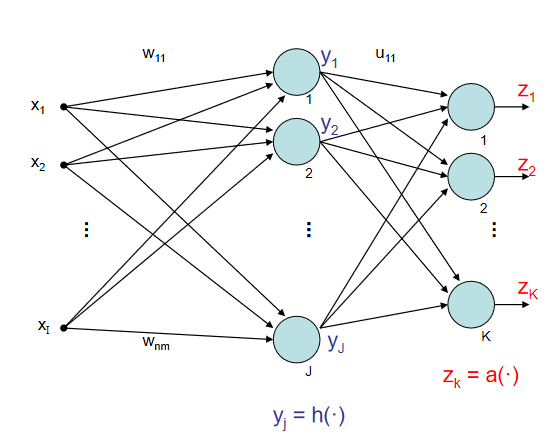
\includegraphics[width=0.9\textwidth]{images/MLP2.png}
          %     \end{figure}
          % \end{column}
        \end{columns}
      \end{frame}

\begin{frame}{Warum "Deep" Learning? -- Mathematische Rechtfertigung für tiefe Netze}
  \begin{columns}
    \begin{column}{1\textwidth}
      \begin{itemize}
        \item \textbf{Representation Learning}: Tiefere Netze lernen hierarchische Merkmalsdarstellungen
        \item \textbf{Mathematischer Vorteil}: Exponentiell weniger Parameter für dieselbe Expressivität
        \item \textbf{Kompositionelle Struktur}: Viele reale Funktionen haben hierarchische Struktur
        \begin{equation}
          f(\mathbf{x}) = g_L(g_{L-1}(...g_2(g_1(\mathbf{x}))...))
        \end{equation}
        \item \textbf{Feature Learning}: Jede Schicht $\ell$ lernt Features der Form:
        \begin{equation}
          \mathbf{h}^{(\ell)} = \sigma(\mathbf{W}^{(\ell)} \mathbf{h}^{(\ell-1)} + \mathbf{b}^{(\ell)})
        \end{equation}
        \item \textbf{Intuition}: 
        \begin{itemize}
          \item Untere Schichten: Einfache Features (Kanten, Texturen)
          \item Mittlere Schichten: Kombinationen (Formen, Teile)
          \item Obere Schichten: Komplexe Konzepte (Objekte, Semantik)
        \end{itemize}
      \end{itemize}
    \end{column}
  \end{columns}
\end{frame}

      \begin{frame}{Das Vanishing Gradient Problem -- Warum tiefe Netze schwer zu trainieren sind}
        \begin{columns}
          \begin{column}{0.6\textwidth}
            \begin{itemize}
              \item \textbf{Problem}: Bei tiefen Netzen werden Gradienten exponentiell kleiner
              \item \textbf{Mathematische Analyse}: Für Sigmoid-Aktivierung $\sigma'(x) \leq 0.25$
              \item Gradient in Schicht $\ell$ proportional zu:
              \begin{equation}
                \frac{\partial L}{\partial \mathbf{W}^{(\ell)}} \propto \prod_{i=\ell+1}^{L} \mathbf{W}^{(i)} \sigma'(\mathbf{z}^{(i)})
              \end{equation}
              \item Für $L-\ell$ Schichten: Faktor $\leq (0.25)^{L-\ell}$ 
              \item \textbf{Beispiel}: Bei 10 Schichten kann Gradient um Faktor $10^{-6}$ schrumpfen!
              \item \textbf{Lösungsansätze}:
              \begin{itemize}
                \item ReLU-Aktivierungen: $\text{ReLU}'(x) = 1$ für $x > 0$
                \item Residual Connections (ResNets)
                \item Normalization (BatchNorm, LayerNorm)
                \item Bessere Initialisierung (Xavier, He)
              \end{itemize}
            \end{itemize}
          \end{column}
           \begin{column}{0.4\textwidth}
             \begin{figure}
               \centering
                           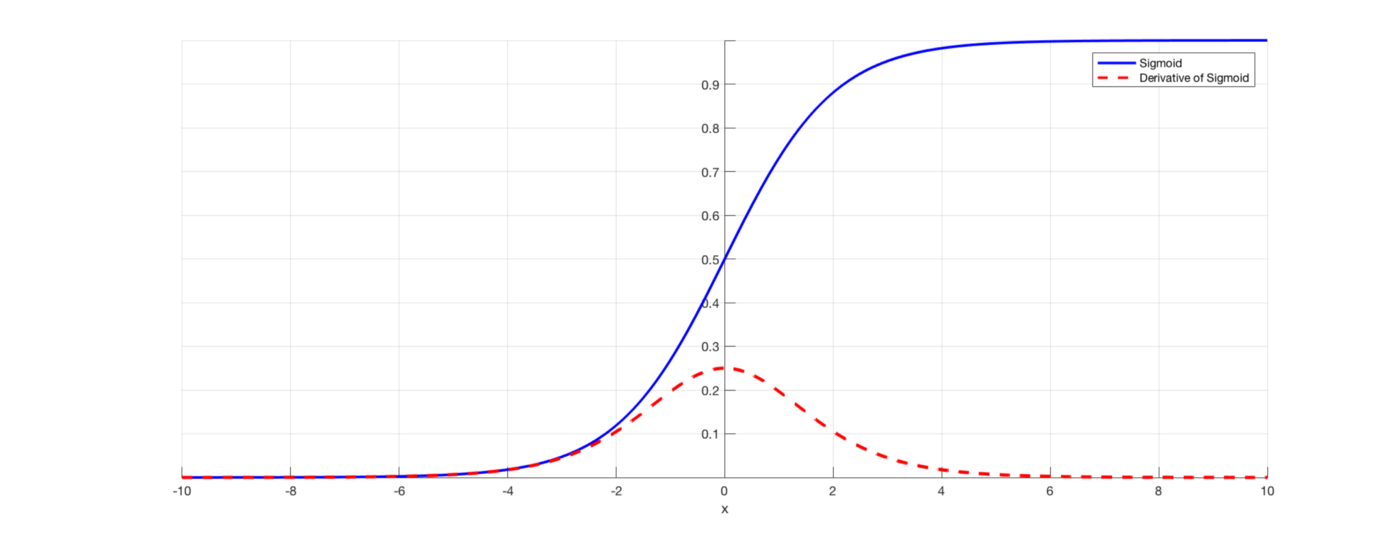
\includegraphics[width=0.9\textwidth]{images/sigmoid.png}
               \end{figure}
           \end{column}
        \end{columns}
      \end{frame}

      \begin{frame}{Aktivierungsfunktionen -- Mathematische Eigenschaften und Warum sie wichtig sind}
        \begin{columns}
          \begin{column}{1\textwidth}
            \begin{itemize}
              \item \textbf{Sigmoid-Funktion}: $\sigma(x) = \frac{1}{1 + e^{-x}}$, Ableitung: $\sigma'(x) = \sigma(x)(1-\sigma(x))$
              \begin{itemize}
                \item Glatt und differenzierbar, Ausgabe in $(0,1)$
                \item \textbf{Problem}: Vanishing Gradients für $|x| >> 0$: $\sigma'(x) \to 0$
              \end{itemize}
              \item \textbf{Tanh-Funktion}: $\tanh(x) = \frac{e^x - e^{-x}}{e^x + e^{-x}}$, Ableitung: $\tanh'(x) = 1 - \tanh^2(x)$
              \begin{itemize}
                \item Ausgabe in $(-1,1)$, zero-centered (bessere Konvergenz)
                \item Ebenfalls Vanishing Gradient Problem
              \end{itemize}
              \item \textbf{ReLU-Funktion} \cite{nair2010}: $\text{ReLU}(x) = \max(0,x)$, Ableitung: $\text{ReLU}'(x) = \begin{cases} 1 & x > 0 \\ 0 & x \leq 0 \end{cases}$
              \begin{itemize}
                \item Löst Vanishing Gradient Problem für $x > 0$
                \item Computationally efficient, führt zu sparse representations
                \item \textbf{Problem}: "Dying ReLU" - Neuronen können "sterben" wenn $x \leq 0$
              \end{itemize}
              \item \textbf{Warum Nichtlinearität essentiell ist}:
              \begin{equation}
                \text{Ohne } \sigma: f(\mathbf{x}) = \mathbf{W}_2(\mathbf{W}_1 \mathbf{x}) = (\mathbf{W}_2\mathbf{W}_1)\mathbf{x} = \mathbf{W}_{\text{linear}}\mathbf{x}
              \end{equation}
            \end{itemize}
          \end{column}
        \end{columns}
      \end{frame}

      \begin{frame}{Häufige Aktivierungsfunktionen -- Visualisierung}
        \begin{columns}
          \begin{column}{0.5\textwidth}
            \begin{figure}
              \centering
                          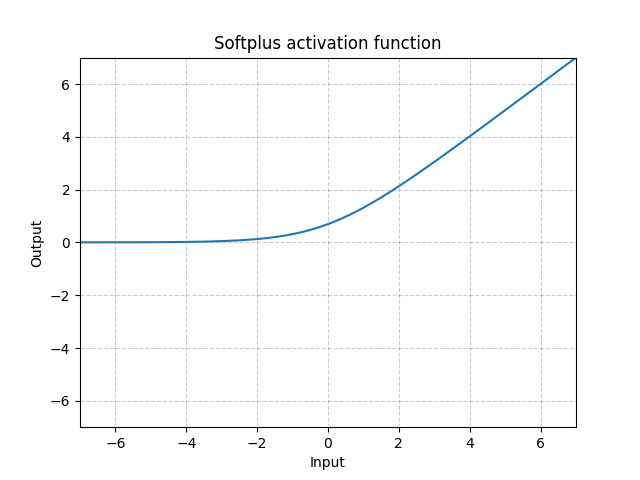
\includegraphics[width=0.9\textwidth]{images/Softplus.png}
              \end{figure}
          \end{column}
           \begin{column}{0.5\textwidth}
             \begin{figure}
               \centering
                           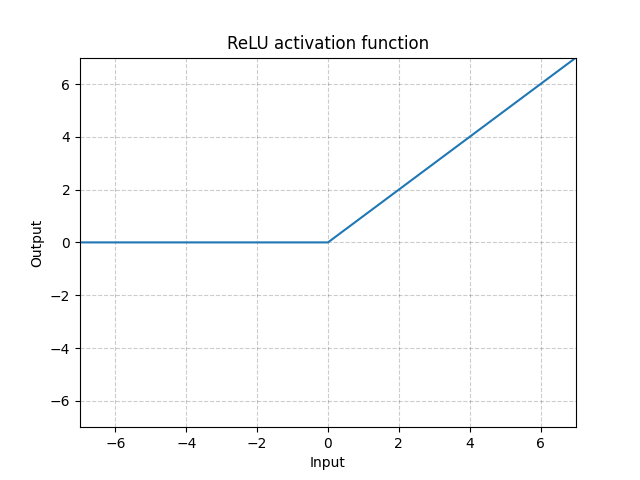
\includegraphics[width=0.9\textwidth]{images/ReLU.png}
               \end{figure}
           \end{column}
        \end{columns}
      \end{frame}

      
      \begin{frame}{Weitere Netzwerk Architekturen}
        \begin{columns}
          \begin{column}{0.6\textwidth}
            \begin{itemize}
              \item spezielle Datenstrukturen profitieren von speziellen Architekturen \newline 
              \item Bilderkennung \rightarrow Convolutional Neural Network (CNN) \newline 
              \item sequentielle Daten \rightarrow Recurrent Neural Networks (RNN) \newline 
              \item im speziellen um Kausalität/Kontext herzustellen \rightarrow Long Short Term Memory (LSTM) \newline
            \end{itemize}
          \end{column}
           \begin{column}{0.4\textwidth}
             \begin{figure}
               \centering
                           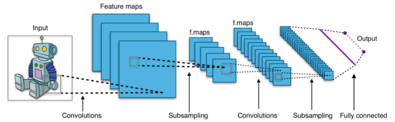
\includegraphics[width=0.9\textwidth]{images/CNN.png}
               \end{figure}
               \begin{figure}
                \centering
                            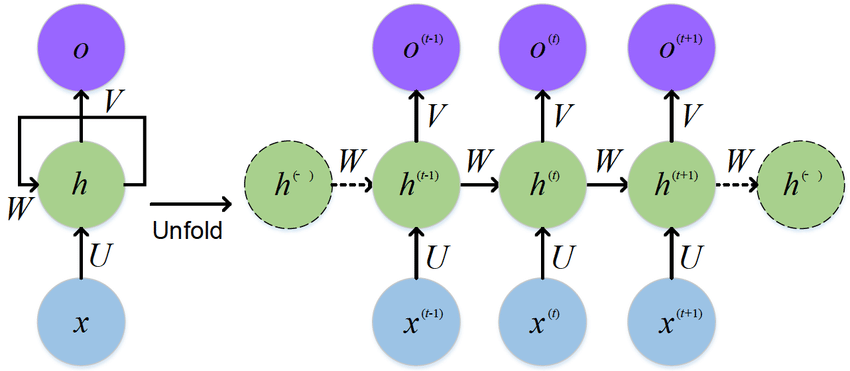
\includegraphics[width=0.9\textwidth]{images/RNN.png}
                \end{figure}
           \end{column}
        \end{columns}
      \end{frame}

      \begin{frame}{Was sind Convolutional Neural Networks (CNNs)?}
        \begin{columns}
          \begin{column}{0.65\textwidth}
            \begin{itemize}
              \item \textbf{CNNs}: Speziell für räumliche Daten entwickelte neuronale Netze
              \item \textbf{Hauptanwendung}: Bildverarbeitung, Computer Vision
              \item \textbf{Grundidee}: Nutze lokale Strukturen in Bildern
              \item \textbf{Kernoperationen}:
              \begin{itemize}
                \item \textbf{Convolution}: Filtere lokale Features
                \item \textbf{Pooling}: Reduziere räumliche Dimensionen
                \item \textbf{Fully Connected}: Klassifikation am Ende
              \end{itemize}
              \item \textbf{Hierarchische Feature-Extraktion}:
              \begin{itemize}
                \item \textbf{Layer 1}: Kanten, Ecken
                \item \textbf{Layer 2}: Texturen, Formen
                \item \textbf{Layer 3}: Objektteile
                \item \textbf{Layer 4}: Vollständige Objekte
              \end{itemize}
              \item \textbf{Vorteil}: Automatisches Lernen relevanter Features
            \end{itemize}
          \end{column}
          \begin{column}{0.35\textwidth}
            \centering
            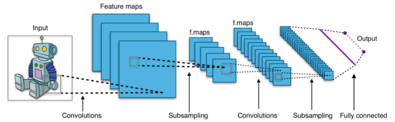
\includegraphics[width=\textwidth]{images/CNN.png}
            \vspace{0.5cm}
            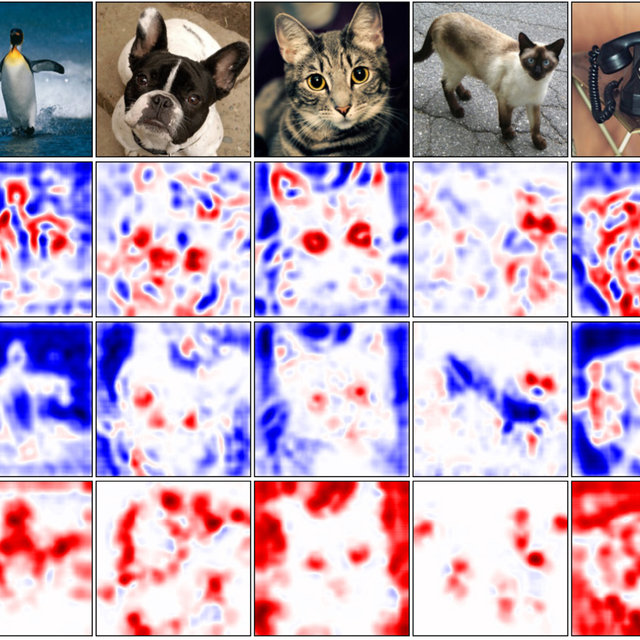
\includegraphics[width=\textwidth]{images/featuremaps.jpg}
          \end{column}
        \end{columns}
      \end{frame}

      \begin{frame}{CNN Grundoperationen: Convolution}
        \begin{columns}
          \begin{column}{0.7\textwidth}
            \begin{itemize}
              \item \textbf{Convolution Operation}:
              \begin{equation}
                (f * g)(x,y) = \sum_{m} \sum_{n} f(m,n) \cdot g(x-m, y-n)
              \end{equation}
              \item \textbf{In CNNs}:
              \begin{equation}
                \text{Output}(i,j) = \sum_{m} \sum_{n} \text{Filter}(m,n) \cdot \text{Input}(i+m, j+n)
              \end{equation}
              \item \textbf{Filter (Kernel)}:
              \begin{itemize}
                \item Kleine Matrizen (z.B. 3×3, 5×5)
                \item Erkennen spezifische Muster
                \item Gewichte werden gelernt
              \end{itemize}
              \item \textbf{Beispiel}: Kantendetektor, Blur-Filter
              \item \textbf{Feature Maps}: Ausgabe nach Convolution + Aktivierung
            \end{itemize}
          \end{column}
          \begin{column}{0.3\textwidth}
            \centering
            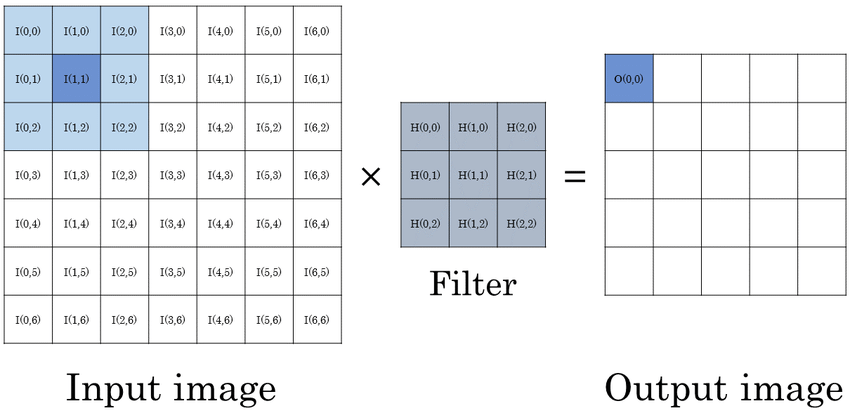
\includegraphics[width=\textwidth]{images/convolution.png}
          \end{column}
        \end{columns}
      \end{frame}
      
      \begin{frame}{Warum funktionieren CNNs? -- Mathematische Prinzipien}
        \begin{columns}
          \begin{column}{1\textwidth}
            \begin{itemize}
              \item \textbf{Drei Schlüsselprinzipien von CNNs}:
              \item \textbf{1. Lokale Konnektivität}: Jedes Neuron ist nur mit lokalem Bereich verbunden
              \begin{equation}
                y_{i,j}^{(\ell)} = \sigma\left(\sum_{m=-k}^{k} \sum_{n=-k}^{k} w_{m,n}^{(\ell)} \cdot x_{i+m,j+n}^{(\ell-1)} + b^{(\ell)}\right)
              \end{equation}
              \item \textbf{2. Parameter Sharing}: Derselbe Filter $\mathbf{W}$ wird über gesamte Feature-Map verwendet
              \begin{itemize}
                \item Reduziert Parameter von $O(H \cdot W \cdot d^2)$ auf $O(k^2 \cdot d)$
                \item Erzwingt Translationsinvarianz
              \end{itemize}
              \item \textbf{3. Equivarianz zu Translationen}: Wenn Input um $\mathbf{t}$ verschoben wird, verschiebt sich Output ebenfalls um $\mathbf{t}$
              \begin{equation}
                \text{Conv}(T_\mathbf{t}[\mathbf{x}]) = T_\mathbf{t}[\text{Conv}(\mathbf{x})]
              \end{equation}
              \item \textbf{Pooling} führt zu begrenzter Translationsinvarianz:
              \begin{equation}
                \text{MaxPool}(\mathbf{X})_{i,j} = \max_{(p,q) \in \mathcal{N}_{i,j}} \mathbf{X}_{p,q}
              \end{equation}
              \item \textbf{Hierarchische Feature-Extraktion}: Einfache → Komplexe Features
            \end{itemize}
          \end{column}
        \end{columns}
      \end{frame}

      \begin{frame}{Spezielle Netzwerkarchitekturen: CNN -- Implementierung}
        \begin{columns}
          \begin{column}{0.6\textwidth}
            \begin{itemize}
              \item \textbf{Convolutional Neural Networks} \cite{lecun1998}: Spezialisiert auf gitterförmige Daten (Bilder) \newline
              \item \textbf{Faltungsoperation} (2D-Convolution):
              \begin{equation}
                (\mathbf{I} * \mathbf{K})_{i,j} = \sum_{m=0}^{M-1} \sum_{n=0}^{N-1} \mathbf{I}_{i+m,j+n} \cdot \mathbf{K}_{m,n}
              \end{equation}
              \item $\mathbf{I}$: Input-Feature-Map, $\mathbf{K}$: Kernel (Filter) der Größe $M \times N$ \newline
              \item \textbf{Pooling}: Dimensionsreduktion, z.B. Max-Pooling:
              \begin{equation}
                \text{MaxPool}(\mathbf{X})_{i,j} = \max_{p,q \in P_{i,j}} \mathbf{X}_{p,q}
              \end{equation}
              \item \textbf{Parameter Sharing}: Derselbe Filter wird über gesamte Feature-Map angewendet
              \item \textbf{Translation Invariance}: Robustheit gegenüber Verschiebungen
            \end{itemize}
          \end{column}
           \begin{column}{0.4\textwidth}
             \begin{figure}
               \centering
                           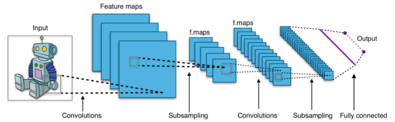
\includegraphics[width=0.9\textwidth]{images/CNN.png}
               \end{figure}
               \begin{figure}
                \centering
                            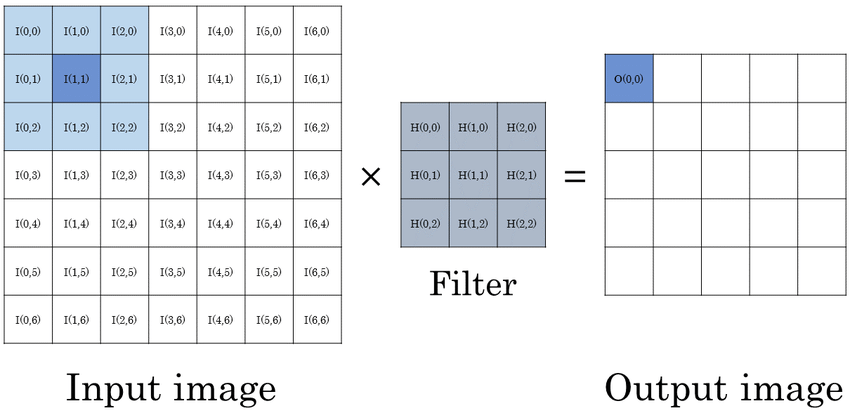
\includegraphics[width=0.9\textwidth]{images/convolution.png}
                \end{figure}
           \end{column}
        \end{columns}
      \end{frame}

      \begin{frame}{Spezielle Netzwerkarchitekturen: CNN}
        \begin{columns}
          \begin{column}{0.5\textwidth}
            \begin{itemize}
              \item Anschaulich: Formen werden erkannt \newline 
              \item Katzenohren sind anders als Hundeohren \newline 
              \item Verallgemeinerbar für andere Objektklassifizierungen \newline
              \item für Details die XAI Vorlesung nächstes Semester
            \end{itemize}
          \end{column}
           \begin{column}{0.5\textwidth}
             \begin{figure}
               \centering
                           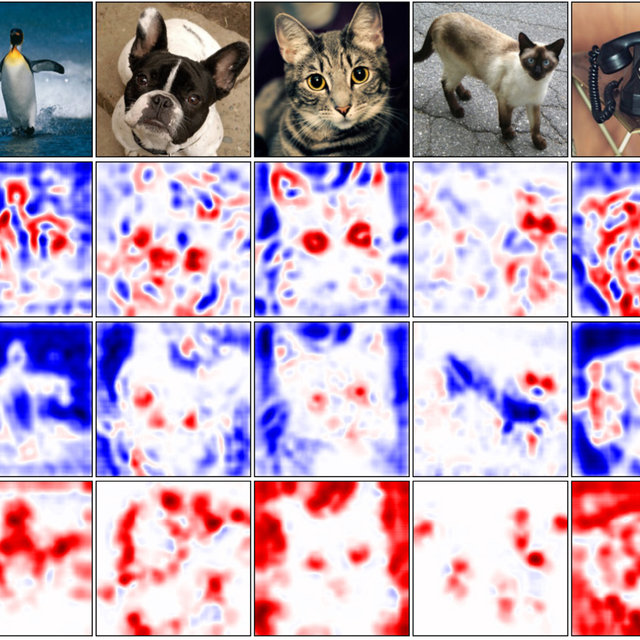
\includegraphics[width=0.9\textwidth]{images/featuremaps.jpg}
               \end{figure}

           \end{column}
        \end{columns}
      \end{frame}

      \begin{frame}{Spezielle Netzwerkarchitekturen: RNN}
        \begin{columns}
          \begin{column}{0.6\textwidth}
            \begin{itemize}
              \item Anschaulich: Schleife in Netzwerk "merkt" sich voherige Zustände \newline 
              \item funktioniert für kurze Zeiträume \newline 
              \item Entfaltung eines RNN \rightarrow viele zu trainierende Gewichte \newline 
              \item Problem: langfristige Zusammenhänge werden nicht erfasst \newline 
              \item Problem: Verschwindende Gradienten
            \end{itemize}
          \end{column}
           \begin{column}{0.4\textwidth}
             \begin{figure}
               \centering
                           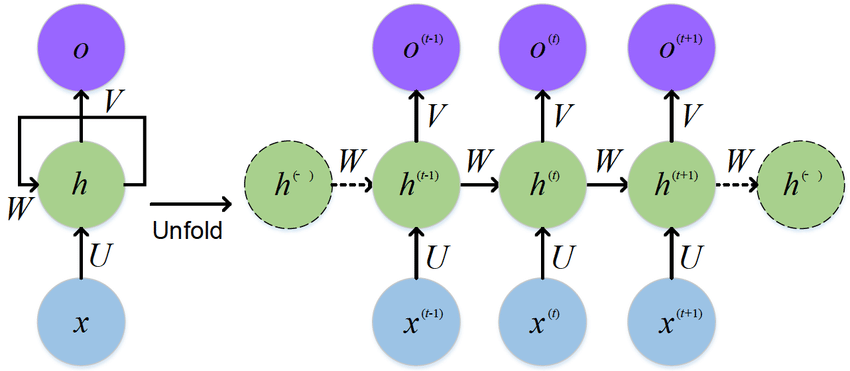
\includegraphics[width=0.9\textwidth]{images/RNN.png}
               \end{figure}

           \end{column}
        \end{columns}
      \end{frame}     
      
      \begin{frame}{Spezielle Netzwerkarchitekturen: LSTM}
        \begin{columns}
          \begin{column}{0.6\textwidth}
            \begin{itemize}
              \item \textbf{Long Short-Term Memory} \cite{hochreiter1997}: Lösung des Vanishing Gradient Problems in RNNs \newline
              \item \textbf{Cell State} $\mathbf{C}_t$: Langzeit-Gedächtnis der LSTM-Zelle \newline
              \item \textbf{Hidden State} $\mathbf{h}_t$: Kurzzeit-Output der Zelle \newline
              \item Drei Gating-Mechanismen kontrollieren Informationsfluss:
              \begin{itemize}
                \item Forget Gate: Welche Informationen vergessen?
                \item Input Gate: Welche neuen Informationen speichern?
                \item Output Gate: Welche Teile des Cell States ausgeben?
              \end{itemize}
            \end{itemize}
          \end{column}
           \begin{column}{0.4\textwidth}
             \begin{figure}
               \centering
                           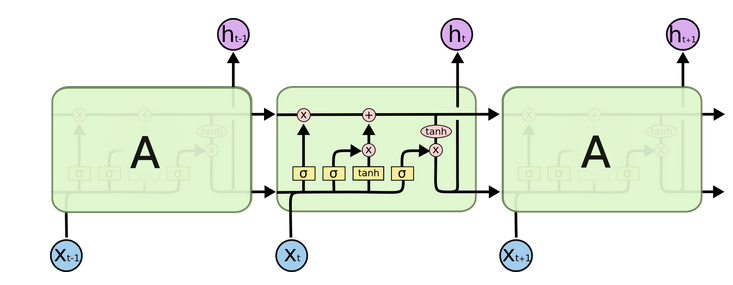
\includegraphics[width=0.9\textwidth]{images/LSTM_1.png}
               \end{figure}
               \begin{figure}
                \centering
                            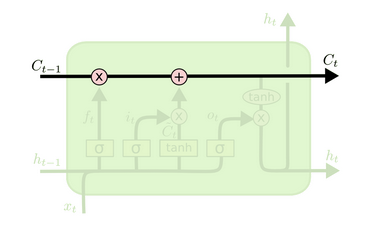
\includegraphics[width=0.9\textwidth]{images/LSTM_2.png}
                \end{figure}

           \end{column}
        \end{columns}
      \end{frame}
      
            
      \begin{frame}{LSTM: Mathematische Formulierung}
        \begin{columns}
          \begin{column}{0.6\textwidth}
            \begin{itemize}              
              \item \textbf{Forget Gate}: Entscheidet, welche Informationen aus $\mathbf{C}_{t-1}$ gelöscht werden
              \begin{equation}
                \mathbf{f}_t = \sigma(\mathbf{W}_f \cdot [\mathbf{h}_{t-1}, \mathbf{x}_t] + \mathbf{b}_f)
              \end{equation}
              \item \textbf{Input Gate}: Bestimmt neue Informationen für Cell State
              \begin{align}
                \mathbf{i}_t &= \sigma(\mathbf{W}_i \cdot [\mathbf{h}_{t-1}, \mathbf{x}_t] + \mathbf{b}_i) \\
                \tilde{\mathbf{C}}_t &= \tanh(\mathbf{W}_C \cdot [\mathbf{h}_{t-1}, \mathbf{x}_t] + \mathbf{b}_C)
              \end{align}
              \item \textbf{Cell State Update}:
              \begin{equation}
                \mathbf{C}_t = \mathbf{f}_t * \mathbf{C}_{t-1} + \mathbf{i}_t * \tilde{\mathbf{C}}_t
              \end{equation}
              \item \textbf{Output Gate} und \textbf{Hidden State}:
              \begin{align}
                \mathbf{o}_t &= \sigma(\mathbf{W}_o \cdot [\mathbf{h}_{t-1}, \mathbf{x}_t] + \mathbf{b}_o) \\
                \mathbf{h}_t &= \mathbf{o}_t * \tanh(\mathbf{C}_t)
              \end{align}
            \end{itemize}
          \end{column}
           \begin{column}{0.4\textwidth}
             \begin{figure}
               \centering
                           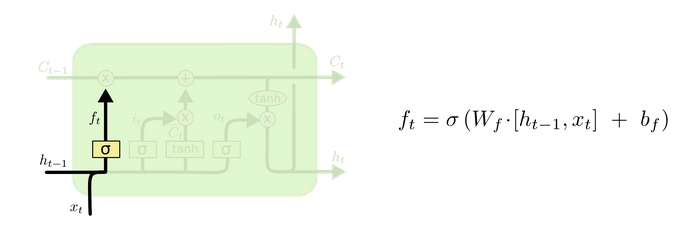
\includegraphics[width=0.9\textwidth]{images/LSTM_3.png}
               \end{figure}
               \begin{figure}
                \centering
                            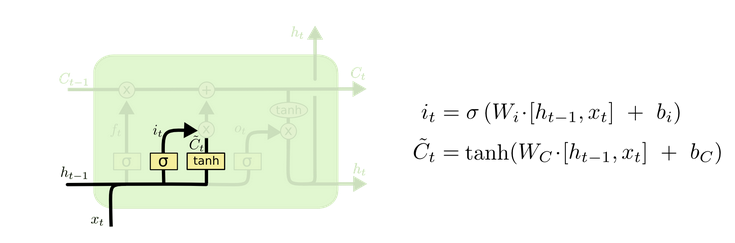
\includegraphics[width=0.9\textwidth]{images/LSTM_4.png}
                \end{figure}
            

           \end{column}
        \end{columns}
      \end{frame} 

      \begin{frame}{LSTM: Cell State Update und Output}
        \begin{columns}
          \begin{column}{0.6\textwidth}
            \begin{itemize}
              \item \textbf{Cell State Update}: Kombination von alten und neuen Informationen
              \begin{equation}
                \mathbf{C}_t = \mathbf{f}_t \odot \mathbf{C}_{t-1} + \mathbf{i}_t \odot \tilde{\mathbf{C}}_t
              \end{equation}
              \item \textbf{Output Gate}: Bestimmt, welche Teile des Cell States ausgegeben werden
              \begin{equation}
                \mathbf{o}_t = \sigma(\mathbf{W}_o \cdot [\mathbf{h}_{t-1}, \mathbf{x}_t] + \mathbf{b}_o)
              \end{equation}
              \item \textbf{Hidden State}: Gefilterte Version des Cell States
              \begin{equation}
                \mathbf{h}_t = \mathbf{o}_t \odot \tanh(\mathbf{C}_t)
              \end{equation}
              \item \textbf{Warum funktioniert LSTM?}
              \begin{itemize}
                \item Cell State kann Informationen über viele Zeitschritte transportieren
                \item Gates kontrollieren selektiv Informationsfluss
                \item Löst das Vanishing Gradient Problem von Standard-RNNs
              \end{itemize}
            \end{itemize}
          \end{column}
           \begin{column}{0.4\textwidth}
               \begin{figure}
                \centering
                            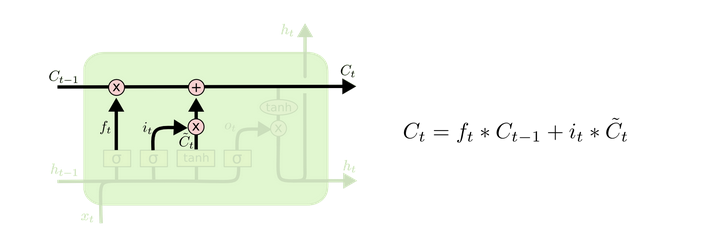
\includegraphics[width=0.9\textwidth]{images/LSTM_5.png}
                \end{figure}
                \begin{figure}
                  \centering
                              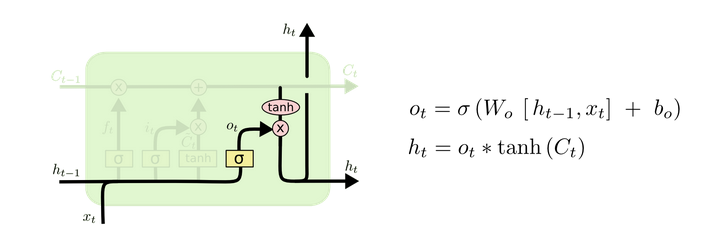
\includegraphics[width=0.9\textwidth]{images/LSTM_6.png}
                  \end{figure}
           \end{column}
        \end{columns}
      \end{frame} 


      \begin{frame}{Autoencoder: Grundlagen und Mathematik}
        \begin{columns}
          \begin{column}{0.6\textwidth}
            \begin{itemize}
              \item \textbf{Autoencoder}: Unsupervised Learning zur Dimensionsreduktion und Rekonstruktion
              \item \textbf{Encoder}: $\mathbf{z} = f_{enc}(\mathbf{x}; \boldsymbol{\theta}_{enc})$ - Komprimierung in latenten Raum
              \item \textbf{Decoder}: $\hat{\mathbf{x}} = f_{dec}(\mathbf{z}; \boldsymbol{\theta}_{dec})$ - Rekonstruktion aus latenter Repräsentation
              \item \textbf{Verlustfunktion}: Rekonstruktionsfehler
              \begin{equation}
                L(\mathbf{x}, \hat{\mathbf{x}}) = ||\mathbf{x} - \hat{\mathbf{x}}||^2
              \end{equation}
              \item \textbf{Latenter Raum} $\mathbf{z} \in \mathbb{R}^d$ mit $d << $ Eingabedimension
              \item \textbf{Anwendungen}:
              \begin{itemize}
                \item Dimensionsreduktion (wie PCA, aber nichtlinear)
                \item Anomaly Detection (hoher Rekonstruktionsfehler)
                \item Denoising (rauschhafte Eingaben, saubere Ziele)
                \item Feature Learning für Downstream-Tasks
              \end{itemize}
            \end{itemize}
          \end{column}
           \begin{column}{0.4\textwidth}
             \begin{figure}
               \centering
                           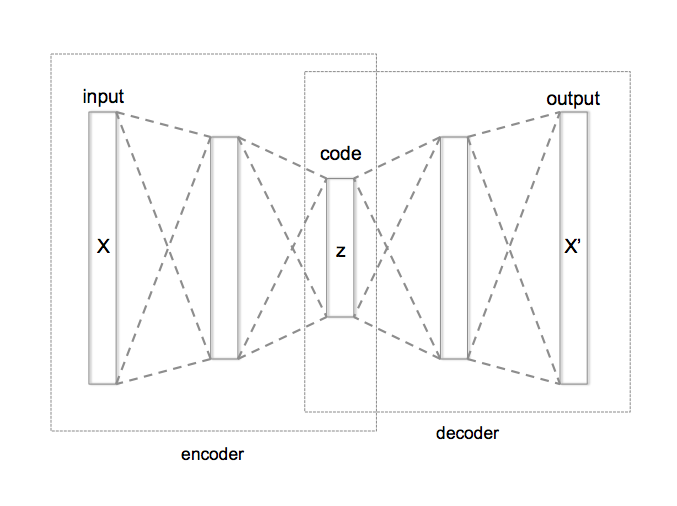
\includegraphics[width=0.9\textwidth]{images/Autoencoder.png}
               \end{figure}
            \end{column}
        \end{columns}
      \end{frame}

\begin{frame}{Variational Autoencoders (VAEs): Motivation}
  \begin{columns}
    \begin{column}{1\textwidth}
      \begin{itemize}
        \item \textbf{Problem klassischer Autoencoders}: Latenter Raum ist nicht interpretierbar oder strukturiert
        \item \textbf{Ziel der VAEs}: Lernen einer \textbf{probabilistischen} latenten Repräsentation
        \item \textbf{Generative Modellierung}: $p(\mathbf{x}) = \int p(\mathbf{x}|\mathbf{z}) p(\mathbf{z}) d\mathbf{z}$
        \item \textbf{Bayessche Perspektive}:
        \begin{itemize}
          \item Prior: $p(\mathbf{z}) = \mathcal{N}(\mathbf{0}, \mathbf{I})$ (Standard-Normalverteilung)
          \item Likelihood: $p(\mathbf{x}|\mathbf{z})$ durch Decoder-Netzwerk
          \item Posterior: $p(\mathbf{z}|\mathbf{x})$ durch Encoder-Netzwerk approximiert
        \end{itemize}
        \item \textbf{Herausforderung}: $p(\mathbf{z}|\mathbf{x})$ ist analytisch nicht berechenbar
        \item \textbf{Lösung}: Variational Inference mit \textbf{Evidence Lower Bound (ELBO)}
        \item \textbf{Vorteil}: Latenter Raum ist \textbf{kontinuierlich} und \textbf{interpolierbar}
        \item \textbf{Anwendungen}: Bildgenerierung, Data Augmentation, Semi-Supervised Learning
      \end{itemize}
    \end{column}
  \end{columns}
\end{frame}

\begin{frame}{VAEs: Mathematische Grundlagen}
  \begin{columns}
    \begin{column}{1\textwidth}
      \begin{itemize}
        \item \textbf{Variational Inference}: Approximiere $p(\mathbf{z}|\mathbf{x})$ durch $q_{\boldsymbol{\phi}}(\mathbf{z}|\mathbf{x})$
        \item \textbf{Evidence Lower Bound (ELBO)}:
        \begin{align}
          \log p(\mathbf{x}) &\geq \mathbb{E}_{q_{\boldsymbol{\phi}}(\mathbf{z}|\mathbf{x})}[\log p_{\boldsymbol{\theta}}(\mathbf{x}|\mathbf{z})] - D_{KL}(q_{\boldsymbol{\phi}}(\mathbf{z}|\mathbf{x}) || p(\mathbf{z}))
        \end{align}
        \item \textbf{Zwei Terme der Verlustfunktion}:
        \begin{itemize}
          \item \textbf{Rekonstruktionsverlust}: $\mathbb{E}_{q_{\boldsymbol{\phi}}(\mathbf{z}|\mathbf{x})}[\log p_{\boldsymbol{\theta}}(\mathbf{x}|\mathbf{z})]$
          \item \textbf{Regularisierungsterm}: $D_{KL}(q_{\boldsymbol{\phi}}(\mathbf{z}|\mathbf{x}) || p(\mathbf{z}))$
        \end{itemize}
        \item \textbf{Encoder}: $q_{\boldsymbol{\phi}}(\mathbf{z}|\mathbf{x}) = \mathcal{N}(\boldsymbol{\mu}_{\boldsymbol{\phi}}(\mathbf{x}), \text{diag}(\boldsymbol{\sigma}_{\boldsymbol{\phi}}^2(\mathbf{x})))$
        \item \textbf{Decoder}: $p_{\boldsymbol{\theta}}(\mathbf{x}|\mathbf{z}) = \mathcal{N}(\boldsymbol{\mu}_{\boldsymbol{\theta}}(\mathbf{z}), \boldsymbol{\sigma}_{\boldsymbol{\theta}}^2 \mathbf{I})$
        \item \textbf{KL-Divergenz} (analytisch berechenbar für Gauß'sche Verteilungen):
        \begin{equation}
          D_{KL} = \frac{1}{2} \sum_{j=1}^{d} (1 + \log(\sigma_j^2) - \mu_j^2 - \sigma_j^2)
        \end{equation}
      \end{itemize}
    \end{column}
  \end{columns}
\end{frame}

\begin{frame}{VAEs: Reparameterization Trick}
  \begin{columns}
    \begin{column}{1\textwidth}
      \begin{itemize}
        \item \textbf{Problem}: Stochastisches Sampling $\mathbf{z} \sim q_{\boldsymbol{\phi}}(\mathbf{z}|\mathbf{x})$ ist nicht differenzierbar
        \item \textbf{Lösung}: Reparameterization Trick (Kingma \& Welling, 2013)
        \item \textbf{Statt}: $\mathbf{z} \sim \mathcal{N}(\boldsymbol{\mu}, \boldsymbol{\sigma}^2)$
        \item \textbf{Verwende}: 
        \begin{align}
          \boldsymbol{\epsilon} &\sim \mathcal{N}(\mathbf{0}, \mathbf{I}) \quad \text{(deterministisches Rauschen)} \\
          \mathbf{z} &= \boldsymbol{\mu} + \boldsymbol{\sigma} \odot \boldsymbol{\epsilon} \quad \text{(deterministische Transformation)}
        \end{align}
        \item \textbf{Vorteil}: Gradienten können durch $\boldsymbol{\mu}$ und $\boldsymbol{\sigma}$ zurückpropagiert werden
        \item \textbf{Praktische Implementierung}:
        \begin{itemize}
          \item Encoder gibt $\boldsymbol{\mu}(\mathbf{x})$ und $\log \boldsymbol{\sigma}^2(\mathbf{x})$ aus
          \item Sample $\boldsymbol{\epsilon} \sim \mathcal{N}(\mathbf{0}, \mathbf{I})$
          \item Berechne $\mathbf{z} = \boldsymbol{\mu} + \exp(\frac{1}{2}\log \boldsymbol{\sigma}^2) \odot \boldsymbol{\epsilon}$
          \item Führe $\mathbf{z}$ durch Decoder
        \end{itemize}
        \item \textbf{Trainingsalgorithmus}: Standard-Backpropagation mit stochastischem Gradienten!
      \end{itemize}
    \end{column}
  \end{columns}
\end{frame}

\begin{frame}{VAEs: Eigenschaften und Anwendungen}
  \begin{columns}
    \begin{column}{1\textwidth}
      \begin{itemize}
        \item \textbf{Interpolation im latenten Raum}: Glatte Übergänge zwischen Datenpunkten
        \begin{equation}
          \mathbf{z}_{interp} = \alpha \mathbf{z}_1 + (1-\alpha) \mathbf{z}_2, \quad \alpha \in [0,1]
        \end{equation}
        \item \textbf{Generierung neuer Daten}: Sample $\mathbf{z} \sim \mathcal{N}(\mathbf{0}, \mathbf{I})$, dann $\mathbf{x}_{new} = \text{Decoder}(\mathbf{z})$
        \item \textbf{Disentangled Representations}: Verschiedene Dimensionen von $\mathbf{z}$ kodieren verschiedene Eigenschaften
        \item \textbf{Anwendungen}:
        \begin{itemize}
          \item \textbf{Computer Vision}: Gesichtsgenerierung, Style Transfer
          \item \textbf{NLP}: Text Generation, Sentence Interpolation
          \item \textbf{Drug Discovery}: Molekularstruktur-Generation
          \item \textbf{Anomaly Detection}: Niedrige Likelihood $\rightarrow$ Anomalie
          \item \textbf{Data Augmentation}: Generierung synthetischer Trainingsdaten
        \end{itemize}
        \item \textbf{Varianten}:
        \begin{itemize}
          \item $\beta$-VAE: $\beta \cdot D_{KL}$ für bessere Disentanglement
          \item Conditional VAE: $p(\mathbf{x}|\mathbf{y}, \mathbf{z})$ mit Labels $\mathbf{y}$
          \item Hierarchical VAE: Mehrere latente Schichten
        \end{itemize}
      \end{itemize}
    \end{column}
  \end{columns}
\end{frame}

\begin{frame}{Generative Adversarial Networks (GANs): Grundprinzip}
  \begin{columns}
    \begin{column}{0.7\textwidth}
      \begin{itemize}
        \item \textbf{Grundidee}: Zwei neuronale Netze konkurrieren miteinander
        \begin{itemize}
          \item \textbf{Generator $G$}: Erzeugt "gefälschte" Daten aus Rauschen
          \item \textbf{Discriminator $D$}: Unterscheidet echte von gefälschten Daten
        \end{itemize}
        \item \textbf{Adversarial Training}: Spieltheoretischer Ansatz
        \begin{align}
          \min_G \max_D V(D,G) = \mathbb{E}_{x \sim p_{data}(x)}[\log D(x)] + \mathbb{E}_{z \sim p_z(z)}[\log(1-D(G(z)))]
        \end{align}
        \item \textbf{Training Process}:
        \begin{enumerate}
          \item \textbf{Discriminator Training}: Maximiere $V(D,G)$
          \begin{itemize}
            \item Lerne echte Daten als "echt" zu klassifizieren
            \item Lerne generierte Daten als "gefälscht" zu erkennen
          \end{itemize}
          \item \textbf{Generator Training}: Minimiere $V(D,G)$
          \begin{itemize}
            \item Erzeuge Daten, die den Discriminator "täuschen"
          \end{itemize}
        \end{enumerate}
      \end{itemize}
    \end{column}
    \begin{column}{0.3\textwidth}
      \centering
      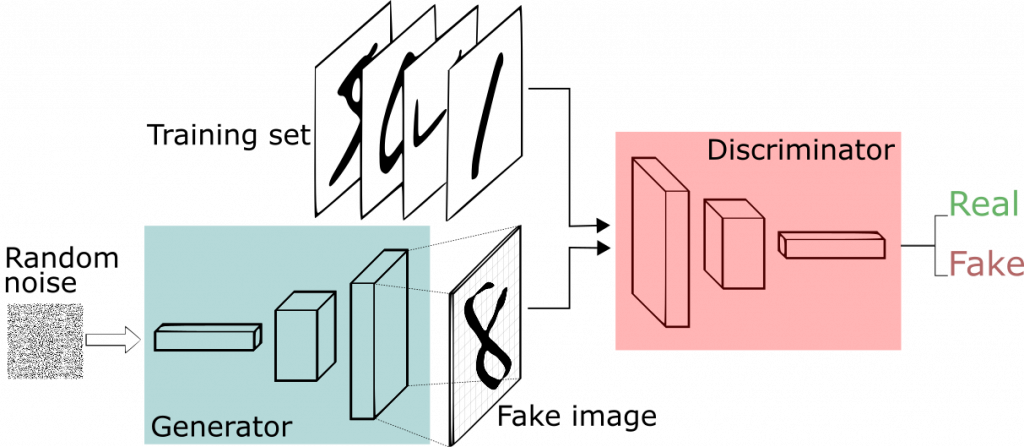
\includegraphics[width=\textwidth]{images/GAN.png}
    \end{column}
  \end{columns}
\end{frame}

\begin{frame}{GAN Training: Mathematische Details}
  \begin{columns}
    \begin{column}{1\textwidth}
      \begin{itemize}
        \item \textbf{Discriminator Loss} (Binary Cross-Entropy):
        \begin{align}
          \mathcal{L}_D = -\mathbb{E}_{x \sim p_{data}}[\log D(x)] - \mathbb{E}_{z \sim p_z}[\log(1-D(G(z)))]
        \end{align}
        \item \textbf{Generator Loss} (Ursprünglich):
        \begin{align}
          \mathcal{L}_G = \mathbb{E}_{z \sim p_z}[\log(1-D(G(z)))]
        \end{align}
        \item \textbf{Problem}: Vanishing Gradients bei schlechtem Generator
        \item \textbf{Praktische Generator Loss} (Non-saturating):
        \begin{align}
          \mathcal{L}_G = -\mathbb{E}_{z \sim p_z}[\log D(G(z))]
        \end{align}
        \item \textbf{Nash-Gleichgewicht}: Theoretisch optimal wenn:
        \begin{align}
          D^*(x) = \frac{p_{data}(x)}{p_{data}(x) + p_g(x)} = \frac{1}{2}
        \end{align}
        wenn $p_g = p_{data}$ (Generator erzeugt perfekte Datenverteilung)
      \end{itemize}
    \end{column}
  \end{columns}
\end{frame}

\begin{frame}{GAN Varianten und Verbesserungen}
  \begin{columns}
    \begin{column}{1\textwidth}
      \begin{itemize}
        \item \textbf{Deep Convolutional GANs (DCGANs)}:
        \begin{itemize}
          \item Verwendung von Convolutional Layers
          \item Batch Normalization, LeakyReLU
          \item Bessere Stabilität für Bildgenerierung
        \end{itemize}
        \item \textbf{Wasserstein GAN (WGAN)}:
        \begin{itemize}
          \item Earth Mover Distance statt JS-Divergenz
          \item Stabileres Training, bessere Konvergenz-Eigenschaften
          \item \textbf{Lipschitz-Constraint}: Kritisch für WGAN-Theorie
        \end{itemize}
        \item \textbf{Conditional GANs (cGANs)}:
        \begin{itemize}
          \item Bedingung auf Labels: $G(z|y)$, $D(x|y)$
          \item Kontrollierte Generierung spezifischer Klassen
        \end{itemize}
        \item \textbf{StyleGAN}:
        \begin{itemize}
          \item Latent Space Manipulation
          \item Progressive Growing, Style Transfer
          \item State-of-the-art für hochauflösende Gesichter
        \end{itemize}
      \end{itemize}
    \end{column}
  \end{columns}
\end{frame}

\begin{frame}{WGAN und die Lipschitz-Constraint: Kurz erklärt}
  \begin{columns}
    \begin{column}{1\textwidth}
      \begin{itemize}
        \item \textbf{Problem bei Standard GANs}: Training instabil, Gradients verschwinden
        \item \textbf{WGAN Lösung}: Verwende Wasserstein-Distanz statt JS-Divergenz
        \item \textbf{Lipschitz-Constraint}: 
        \begin{itemize}
          \item \textbf{Einfach gesagt}: Discriminator darf nicht "zu steil" werden
          \item \textbf{Mathematisch}: $|f(x_1) - f(x_2)| \leq L \cdot |x_1 - x_2|$
          \item \textbf{Warum nötig?} Wasserstein-Distanz erfordert beschränkte Funktionen
        \end{itemize}
        \item \textbf{Praktische Umsetzung}:
        \begin{itemize}
          \item \textbf{Weight Clipping}: Einfach, aber problematisch
          \item \textbf{Gradient Penalty}: Moderne Lösung - bestraft zu steile Gradienten
          \item \textbf{Spectral Normalization}: Normalisiert Netzwerk-Gewichte
        \end{itemize}
        \item \textbf{Resultat}: Stabileres Training, bessere Konvergenz
        \item \textbf{Take-away}: Theoretische Constraints führen zu praktischen Verbesserungen
      \end{itemize}
    \end{column}
  \end{columns}
\end{frame}

\begin{frame}{GAN Herausforderungen und Lösungsansätze}
  \begin{columns}
    \begin{column}{1\textwidth}
      \begin{itemize}
        \item \textbf{Training Instabilität}:
        \begin{itemize}
          \item \textbf{Problem}: Discriminator wird zu gut $\rightarrow$ Generator bekommt keine Gradienten
          \item \textbf{Lösung}: Balanced Training, Learning Rate Scheduling
        \end{itemize}
        \item \textbf{Mode Collapse}:
        \begin{itemize}
          \item \textbf{Problem}: Generator erzeugt nur wenige Modi der Datenverteilung
          \item \textbf{Lösung}: Unrolled GANs, Diversity-encouraging Loss Terms
        \end{itemize}
        \item \textbf{Evaluation Metrics}:
        \begin{itemize}
          \item \textbf{Inception Score (IS)}: Misst Bildqualität und Diversität
          \item \textbf{Fréchet Inception Distance (FID)}: Vergleicht Feature-Statistiken
          \item \textbf{Precision \& Recall}: Qualität vs. Diversität Trade-off
        \end{itemize}
        \item \textbf{Praktische Tipps}:
        \begin{itemize}
          \item Feature Matching, Experience Replay
          \item Spectral Normalization, Self-Attention
          \item Progressive Growing für hohe Auflösungen
        \end{itemize}
      \end{itemize}
    \end{column}
  \end{columns}
\end{frame}

\begin{frame}{GANs vs. VAEs: Vergleich der generativen Modelle}
  \begin{columns}
    \begin{column}{1\textwidth}
      \begin{itemize}
        \item \textbf{Generative Adversarial Networks (GANs)}:
        \begin{itemize}
          \item Adversarial Training: Generator vs. Discriminator
          \item Sehr scharfe, realistische Bilder
          \item Training instabil, Mode Collapse möglich
          \item Kein Encoder - keine direkte latente Repräsentation von Daten
        \end{itemize}
        \item \textbf{Variational Autoencoders (VAEs)}:
        \begin{itemize}
          \item Likelihood-basiertes Training mit ELBO
          \item Verschwommene Bilder durch Gauss-Annahme
          \item Stabiles Training, theoretisch fundiert
          \item Bidirektional: Encoding und Decoding möglich
        \end{itemize}
        \item \textbf{Praktische Wahl}:
        \begin{itemize}
          \item \textbf{GANs}: Wenn Bildqualität wichtigster Faktor
          \item \textbf{VAEs}: Wenn interpretierbare latente Repräsentation wichtig
          \item \textbf{Hybrid-Modelle}: VAE-GAN kombiniert beide Ansätze
        \end{itemize}
      \end{itemize}
    \end{column}
  \end{columns}
\end{frame} 

\begin{frame}{Wann Deep Learning? Wann klassisches Machine Learning?}
  \begin{columns}
    \begin{column}{1\textwidth}
      \begin{itemize}
        \item \textbf{Deep Learning ist sinnvoll bei}:
        \begin{itemize}
          \item \textbf{Große Datenmengen}: > 10.000 Samples (je mehr, desto besser)
          \item \textbf{Komplexe Muster}: Bilder, Audio, Text, Sequenzen
          \item \textbf{Hierarchische Strukturen}: Features müssen automatisch gelernt werden
          \item \textbf{Raw Data}: Wenig/keine Feature-Engineering nötig
          \item \textbf{End-to-End Learning}: Von Rohdaten zur Entscheidung
          \item \textbf{Ausreichend Rechenkapazität}: GPUs verfügbar
        \end{itemize}
        \item \textbf{Klassisches ML ist besser bei}:
        \begin{itemize}
          \item \textbf{Kleine Datenmengen}: < 1.000 Samples
          \item \textbf{Strukturierte/tabellarische Daten}: Features sind bereits bekannt
          \item \textbf{Interpretierbarkeit wichtig}: Entscheidungen müssen erklärbar sein
          \item \textbf{Schnelle Inferenz}: Real-time Anwendungen mit Latenz-Constraints
          \item \textbf{Begrenzte Ressourcen}: Wenig Rechenleistung/Speicher
          \item \textbf{Gut definierte Features}: Domain-Wissen kann genutzt werden
        \end{itemize}
      \end{itemize}
    \end{column}
  \end{columns}
\end{frame}

\begin{frame}{Praktische Entscheidungshilfe: Deep Learning vs. klassisches ML}
  \begin{columns}
    \begin{column}{1\textwidth}
      \begin{itemize}
        \item \textbf{Beispiele für Deep Learning}:
        \begin{itemize}
          \item \textbf{Computer Vision}: Objekterkennung, medizinische Bildanalyse
          \item \textbf{NLP}: Sprachübersetzung, Chatbots, Sentiment Analysis
          \item \textbf{Predictive Maintenance}: Sensordaten, Zeitreihen mit vielen Features
          \item \textbf{Generative Tasks}: Bild-/Texterstellung, Data Augmentation
        \end{itemize}
        \item \textbf{Beispiele für klassisches ML}:
        \begin{itemize}
          \item \textbf{Tabellarische Daten}: Kreditscoring, Kundenklassifikation
          \item \textbf{Einfache Klassifikation}: Mit wenigen, gut verstandenen Features
          \item \textbf{Regression}: Preisvorhersage, wissenschaftliche Analysen
          \item \textbf{Clustering}: Kundensegmentierung, Anomalieerkennung
        \end{itemize}
        \item \textbf{Hybride Ansätze}:
        \begin{itemize}
          \item \textbf{Feature-Extraktion}: Deep Learning für Features + klassisches ML für Klassifikation
          \item \textbf{Ensemble}: Kombination verschiedener Ansätze
          \item \textbf{Transfer Learning}: Pretrained Models + Domain-spezifische Anpassung
        \end{itemize}
        \item \textbf{Praktischer Tipp}: Beginne mit einfachsten Methoden, steigere Komplexität schrittweise
      \end{itemize}
    \end{column}
  \end{columns}
\end{frame}



\begin{frame}{Zusammenfassung: Was haben wir gelernt?}
  \begin{columns}
    \begin{column}{1\textwidth}
      \begin{itemize}
        \item \textbf{Mathematische Grundlagen}: Lineare Algebra, Gradienten, Optimierung als Fundament
        \item \textbf{Perceptron bis Deep Learning}: Von linearer Separierung zum Universal Approximation Theorem
        \item \textbf{Training neuronaler Netze}: Backpropagation, Gradientenabstieg, moderne Optimierer (ADAM)
        \item \textbf{Warum Deep Learning funktioniert}: Hierarchische Features, Komposition, Expressivität
        \item \textbf{Herausforderungen}: Vanishing Gradients, Aktivierungsfunktionen, Regularisierung
        \item \textbf{Spezielle Architekturen}:
        \begin{itemize}
          \item \textbf{CNNs}: Translation Equivarianz für Bilddaten
          \item \textbf{RNNs/LSTMs}: Sequentielle Daten und Langzeit-Gedächtnis
          \item \textbf{VAEs}: Probabilistische latente Repräsentationen
          \item \textbf{GANs}: Adversarial Training für realistische Daten
        \end{itemize}
      \end{itemize}
    \end{column}
  \end{columns}
\end{frame}

\begin{frame}{Zentrale Erkenntnisse und Ausblick}
  \begin{columns}
    \begin{column}{1\textwidth}
      \begin{itemize}
        \item \textbf{Theoretisches Verständnis ist entscheidend}:
        \begin{itemize}
          \item Neuronale Netze sind nicht "Black Boxes" - mathematisch fundiert
          \item Universal Approximation erklärt das Potenzial
          \item Gradient Flow erklärt Trainierbarkeit
        \end{itemize}
        \item \textbf{Architektur-Wahl ist problemspezifisch}:
        \begin{itemize}
          \item Nicht immer ist "Deep Learning" die beste Lösung
          \item Inductive Biases nutzen (CNNs für Bilder, RNNs für Sequenzen)
          \item Trade-offs zwischen Komplexität und Interpretierbarkeit
        \end{itemize}
        \item \textbf{Praktische Anwendung erfordert}:
        \begin{itemize}
          \item Datenqualität und -quantität
          \item Richtige Problemformulierung
          \item Evaluation und Validierung
          \item Domain-Wissen einbeziehen
        \end{itemize}
        \item \textbf{Zukunft}: Transformer, Attention, Self-Supervised Learning, Foundation Models
        \item \textbf{Ethik}: Verantwortlicher Einsatz, Bias, Interpretierbarkeit, Nachhaltigkeit
      \end{itemize}
    \end{column}
  \end{columns}
\end{frame}



\begin{frame}[allowframebreaks]{References}
 \bibliographystyle{ieeetr}
 \bibliography{lit.bib}
\end{frame}
\end{document}
